%% Soft Computing (Springer) submission -- Springer Nature LaTeX template (sn-jnl.cls).
%% Compiles directly on Overleaf (fallback layout via sn-compat.tex). For the exact
%% Springer layout add sn-jnl.cls and sn-basic.bst from Overleaf's official
%% "Springer Nature LaTeX Template" (see README.txt).
% If the Springer Nature class is present (official Overleaf template), use it;
% otherwise fall back to a compatible layout so the project compiles anywhere.
\IfFileExists{sn-jnl.cls}{%
  \documentclass[pdflatex,sn-basic]{sn-jnl}% author-year references (Springer basic)
}{%
  \documentclass[11pt]{article}
  % sn-compat.tex -- used only when sn-jnl.cls is not available.
% Provides the Springer Nature front-matter commands on top of article.cls so that
% the manuscript compiles unchanged; the layout approximates a single-column
% Springer submission. Remove nothing: with sn-jnl.cls present this file is ignored.
\usepackage[T1]{fontenc}
\usepackage[a4paper,margin=2.5cm]{geometry}
\usepackage[authoryear,round]{natbib}
\bibliographystyle{plainnat}
\usepackage[hidelinks]{hyperref}
\usepackage{setspace}
\onehalfspacing
\makeatletter
\newcommand{\fnm}[1]{#1}
\newcommand{\sur}[1]{#1}
\newcommand{\orgdiv}[1]{#1}
\newcommand{\orgname}[1]{#1}
\newcommand{\orgaddress}[1]{#1}
\newcommand{\city}[1]{#1}
\newcommand{\country}[1]{#1}
\newcommand{\email}[1]{\gdef\sn@email{#1}}
\gdef\sn@email{}
\gdef\sn@affil{}
\def\author{\@ifstar{\sn@author}{\sn@author}}
\def\sn@author[#1]#2{\gdef\@author{#2}}
\newcommand{\affil}{\@ifstar{\sn@affilcmd}{\sn@affilcmd}}
\def\sn@affilcmd[#1]#2{\gdef\sn@affil{#2}}
\renewcommand{\title}[2][]{\gdef\@title{#2}}
\renewcommand{\abstract}[1]{\gdef\sn@abstract{#1}}
\newcommand{\keywords}[1]{\gdef\sn@keywords{#1}}
\renewcommand{\maketitle}{%
  \begin{center}
    {\Large\bfseries\@title\par}\vspace{1em}
    {\large\@author\textsuperscript{*}\par}\vspace{0.4em}
    {\small\sn@affil\par
     \textsuperscript{*}Corresponding author. E-mail: \texttt{\sn@email}\par}
  \end{center}
  \vspace{1em}
  \noindent\textbf{Abstract.} \sn@abstract\par\medskip
  \noindent\textbf{Keywords:} \sn@keywords\par\bigskip}
\newcommand{\backmatter}{}
\newcommand{\bmhead}[1]{\paragraph*{#1}}
\makeatother

}

\usepackage{graphicx}
\usepackage{multirow}
\usepackage{amsmath,amssymb,amsfonts}
\usepackage{amsthm}
\usepackage{mathrsfs}
\usepackage{xcolor}
\usepackage{booktabs}
\usepackage{tikz}
\usetikzlibrary{positioning,arrows.meta,fit,backgrounds,calc}
\IfFileExists{xurl.sty}{\usepackage{xurl}}{}

\theoremstyle{plain}
\newtheorem{proposition}{Proposition}
\newtheorem{lemma}{Lemma}
\theoremstyle{remark}
\newtheorem{remark}{Remark}

\graphicspath{{fig/}}
% generated by src/make_latex.py -- do not edit by hand
\newcommand{\Ntotal}{23,218}
\newcommand{\Nusers}{16,010}
\newcommand{\Nage}{15,888}
\newcommand{\Ncomplete}{12,206}
\newcommand{\Nfinal}{11,920}
\newcommand{\Nstraight}{286}
\newcommand{\Ncountries}{92}
\newcommand{\AgeMean}{22.9}
\newcommand{\AgeSD}{6.1}
\newcommand{\ChiSq}{9,046.7}
\newcommand{\CfaDf}{271}
\newcommand{\CFIval}{0.940}
\newcommand{\TLIval}{0.928}
\newcommand{\RMSEAval}{0.052}
\newcommand{\SRMRval}{0.046}
\newcommand{\HTMTmax}{0.81}
\newcommand{\Harman}{30.5}
\newcommand{\TRFSmean}{50.5}
\newcommand{\TRFSsd}{19.7}
\newcommand{\TRFSmedian}{50.0}
\newcommand{\PctHuman}{25.8}
\newcommand{\PctPartial}{46.1}
\newcommand{\PctFull}{28.1}
\newcommand{\KWusageH}{1,116.7}
\newcommand{\RhoUsage}{0.30}
\newcommand{\PCmean}{61.2}
\newcommand{\PCsd}{16.1}
\newcommand{\IQmean}{58.6}
\newcommand{\IQsd}{16.7}
\newcommand{\TWmean}{49.8}
\newcommand{\TWsd}{20.4}
\newcommand{\RhoTSI}{0.39}
\newcommand{\RhoSat}{0.55}
\newcommand{\RhoExp}{0.45}
\newcommand{\RhoUse}{0.30}
\newcommand{\RhoReplace}{-0.013}
\newcommand{\PReplace}{0.16}
\newcommand{\FriedmanChi}{5,164.5}
\newcommand{\KendallW}{0.048}
\newcommand{\AnnRMSE}{21.61}
\newcommand{\AnnMAE}{17.39}
\newcommand{\AnnRsq}{0.259}
\newcommand{\HybRMSE}{21.67}
\newcommand{\HybMAE}{17.45}
\newcommand{\HybRsq}{0.255}
\newcommand{\HybP}{=0.013}
\newcommand{\GbRMSE}{21.62}
\newcommand{\GbMAE}{17.32}
\newcommand{\GbRsq}{0.259}
\newcommand{\GbP}{=0.975}
\newcommand{\RfRMSE}{21.67}
\newcommand{\RfMAE}{17.33}
\newcommand{\RfRsq}{0.255}
\newcommand{\RfP}{=0.204}
\newcommand{\LrRMSE}{21.72}
\newcommand{\LrMAE}{17.53}
\newcommand{\LrRsq}{0.252}
\newcommand{\LrP}{=0.003}
\newcommand{\SvrRMSE}{21.86}
\newcommand{\SvrMAE}{17.33}
\newcommand{\SvrRsq}{0.242}
\newcommand{\SvrP}{<0.001}
\newcommand{\FisRMSE}{23.10}
\newcommand{\FisMAE}{18.70}
\newcommand{\FisRsq}{0.155}
\newcommand{\FisP}{<0.001}
\newcommand{\CVsplits}{10}
\newcommand{\CVrepeats}{3}
\newcommand{\CVfits}{30}
\newcommand{\FisShare}{60}
\newcommand{\AnnFisRatio}{1.7}
\newcommand{\LoadMin}{0.53}
\newcommand{\PhiEmax}{0.20}
\newcommand{\SurrRsq}{0.955}
\newcommand{\SurrRMSE}{4.19}
\newcommand{\ImpTau}{0.21}
\newcommand{\RobDraws}{500}
\newcommand{\RobTau}{0.953}
\newcommand{\RobTauLow}{0.911}
\newcommand{\RobAgree}{99.5}
\newcommand{\RobAgreeMin}{80}
\newcommand{\EpsMax}{0.009}
\newcommand{\EpsVersion}{0.009}
\newcommand{\ImpTE}{0.020}
\newcommand{\SensTE}{0.58}
\newcommand{\RhoTE}{0.20}
\newcommand{\ImpSE}{0.045}
\newcommand{\SensSE}{0.67}
\newcommand{\RhoSE}{0.35}
\newcommand{\ImpP}{0.045}
\newcommand{\SensP}{1.04}
\newcommand{\RhoP}{0.39}
\newcommand{\ImpAC}{0.075}
\newcommand{\SensAC}{1.31}
\newcommand{\RhoAC}{0.40}
\newcommand{\ImpC}{0.003}
\newcommand{\SensC}{0.98}
\newcommand{\RhoC}{0.16}
\newcommand{\ImpA}{0.016}
\newcommand{\SensA}{1.20}
\newcommand{\RhoA}{0.28}
\newcommand{\ImpR}{0.094}
\newcommand{\SensR}{6.46}
\newcommand{\RhoR}{0.36}
\newcommand{\ImpE}{0.008}
\newcommand{\SensE}{3.49}
\newcommand{\RhoE}{0.09}
\makeatletter
\expandafter\def\csname act@A1@score\endcsname{54.7}
\expandafter\def\csname act@A1@lo\endcsname{54.3}
\expandafter\def\csname act@A1@hi\endcsname{55.0}
\expandafter\def\csname act@A1@full\endcsname{31.6}
\expandafter\def\csname act@A1@human\endcsname{16.3}
\expandafter\def\csname act@A1@cap\endcsname{3.80}
\expandafter\def\csname act@A1@rank\endcsname{1}
\expandafter\def\csname act@A1@tier\endcsname{AI-leaning}
\expandafter\def\csname act@A2@score\endcsname{53.3}
\expandafter\def\csname act@A2@lo\endcsname{52.9}
\expandafter\def\csname act@A2@hi\endcsname{53.6}
\expandafter\def\csname act@A2@full\endcsname{28.7}
\expandafter\def\csname act@A2@human\endcsname{17.9}
\expandafter\def\csname act@A2@cap\endcsname{3.65}
\expandafter\def\csname act@A2@rank\endcsname{2}
\expandafter\def\csname act@A2@tier\endcsname{AI-leaning}
\expandafter\def\csname act@A5@score\endcsname{50.9}
\expandafter\def\csname act@A5@lo\endcsname{50.6}
\expandafter\def\csname act@A5@hi\endcsname{51.3}
\expandafter\def\csname act@A5@full\endcsname{22.2}
\expandafter\def\csname act@A5@human\endcsname{20.4}
\expandafter\def\csname act@A5@cap\endcsname{3.46}
\expandafter\def\csname act@A5@rank\endcsname{3}
\expandafter\def\csname act@A5@tier\endcsname{AI-leaning}
\expandafter\def\csname act@A3@score\endcsname{50.3}
\expandafter\def\csname act@A3@lo\endcsname{49.9}
\expandafter\def\csname act@A3@hi\endcsname{50.6}
\expandafter\def\csname act@A3@full\endcsname{24.1}
\expandafter\def\csname act@A3@human\endcsname{23.9}
\expandafter\def\csname act@A3@cap\endcsname{3.42}
\expandafter\def\csname act@A3@rank\endcsname{4}
\expandafter\def\csname act@A3@tier\endcsname{Balanced}
\expandafter\def\csname act@A4@score\endcsname{49.4}
\expandafter\def\csname act@A4@lo\endcsname{49.0}
\expandafter\def\csname act@A4@hi\endcsname{49.7}
\expandafter\def\csname act@A4@full\endcsname{20.3}
\expandafter\def\csname act@A4@human\endcsname{23.6}
\expandafter\def\csname act@A4@cap\endcsname{3.36}
\expandafter\def\csname act@A4@rank\endcsname{5}
\expandafter\def\csname act@A4@tier\endcsname{Human-leaning}
\expandafter\def\csname act@A6@score\endcsname{49.1}
\expandafter\def\csname act@A6@lo\endcsname{48.7}
\expandafter\def\csname act@A6@hi\endcsname{49.4}
\expandafter\def\csname act@A6@full\endcsname{20.1}
\expandafter\def\csname act@A6@human\endcsname{24.0}
\expandafter\def\csname act@A6@cap\endcsname{3.32}
\expandafter\def\csname act@A6@rank\endcsname{6}
\expandafter\def\csname act@A6@tier\endcsname{Human-leaning}
\expandafter\def\csname act@A8@score\endcsname{48.6}
\expandafter\def\csname act@A8@lo\endcsname{48.2}
\expandafter\def\csname act@A8@hi\endcsname{48.9}
\expandafter\def\csname act@A8@full\endcsname{21.7}
\expandafter\def\csname act@A8@human\endcsname{26.7}
\expandafter\def\csname act@A8@cap\endcsname{3.27}
\expandafter\def\csname act@A8@rank\endcsname{7}
\expandafter\def\csname act@A8@tier\endcsname{Human-leaning}
\expandafter\def\csname act@A10@score\endcsname{48.1}
\expandafter\def\csname act@A10@lo\endcsname{47.8}
\expandafter\def\csname act@A10@hi\endcsname{48.5}
\expandafter\def\csname act@A10@full\endcsname{16.5}
\expandafter\def\csname act@A10@human\endcsname{23.1}
\expandafter\def\csname act@A10@cap\endcsname{3.18}
\expandafter\def\csname act@A10@rank\endcsname{8}
\expandafter\def\csname act@A10@tier\endcsname{Human-leaning}
\expandafter\def\csname act@A7@score\endcsname{48.1}
\expandafter\def\csname act@A7@lo\endcsname{47.8}
\expandafter\def\csname act@A7@hi\endcsname{48.5}
\expandafter\def\csname act@A7@full\endcsname{16.1}
\expandafter\def\csname act@A7@human\endcsname{23.5}
\expandafter\def\csname act@A7@cap\endcsname{3.23}
\expandafter\def\csname act@A7@rank\endcsname{9}
\expandafter\def\csname act@A7@tier\endcsname{Human-leaning}
\expandafter\def\csname act@A9@score\endcsname{46.5}
\expandafter\def\csname act@A9@lo\endcsname{46.2}
\expandafter\def\csname act@A9@hi\endcsname{46.9}
\expandafter\def\csname act@A9@full\endcsname{19.0}
\expandafter\def\csname act@A9@human\endcsname{31.1}
\expandafter\def\csname act@A9@cap\endcsname{3.14}
\expandafter\def\csname act@A9@rank\endcsname{10}
\expandafter\def\csname act@A9@tier\endcsname{Human-leaning}
\newcommand{\act}[2]{\csname act@#1@#2\endcsname}
\makeatother

% generated by src/make_latex.py (extended analyses) -- do not edit by hand
\newcommand{\cLval}{18.57}
\newcommand{\cHval}{81.43}
\newcommand{\cLnum}{18.571}
\newcommand{\FlatRules}{6,561}
\newcommand{\HierRules}{126}
\newcommand{\RuleReduction}{98.1}
\newcommand{\MamWorst}{2.70}
\newcommand{\MamShare}{9.4}
\newcommand{\RhoMamWa}{0.981}
\newcommand{\RMamWa}{0.979}
\newcommand{\RhoWaTSI}{0.38}
\newcommand{\WaMean}{49.2}
\newcommand{\WaSD}{22.0}
\newcommand{\WaTau}{0.96}
\newcommand{\WaMax}{54.2}
\newcommand{\WaMin}{45.7}
\newcommand{\ShapRsq}{0.255}
\newcommand{\ShapB}{500}
\newcommand{\ShapAC}{0.064}
\newcommand{\ShapPctAC}{25.2}
\newcommand{\ShapR}{0.055}
\newcommand{\ShapPctR}{21.7}
\newcommand{\ShapP}{0.054}
\newcommand{\ShapPctP}{21.2}
\newcommand{\ShapSE}{0.045}
\newcommand{\ShapPctSE}{17.6}
\newcommand{\ShapA}{0.020}
\newcommand{\ShapPctA}{8.0}
\newcommand{\ShapTE}{0.009}
\newcommand{\ShapPctTE}{3.5}
\newcommand{\ShapC}{0.005}
\newcommand{\ShapPctC}{1.9}
\newcommand{\ShapE}{0.002}
\newcommand{\ShapPctE}{0.8}
\newcommand{\MlN}{11,586}
\newcommand{\MlCountries}{50}
\newcommand{\MlMinN}{30}
\newcommand{\IccTSI}{0.084}
\newcommand{\IccTRFS}{0.090}
\newcommand{\IccCond}{0.051}
\newcommand{\RsqMarg}{0.239}
\newcommand{\RsqCond}{0.278}
\newcommand{\LRval}{342.7}
\newcommand{\BetaTE}{-1.94}
\newcommand{\BetaSE}{3.65}
\newcommand{\BetaP}{2.98}
\newcommand{\BetaAC}{4.65}
\newcommand{\BetaC}{-0.49}
\newcommand{\BetaA}{1.49}
\newcommand{\BetaR}{4.38}
\newcommand{\BetaE}{-0.02}
\newcommand{\QolsBeta}{5.03}
\newcommand{\QbetaTen}{4.90}
\newcommand{\QbetaFifty}{5.73}
\newcommand{\QbetaNinety}{4.94}
\newcommand{\QReps}{20}
\newcommand{\TostDelta}{2}
\newcommand{\TostN}{5}
\newcommand{\Dmax}{0.25}
\newcommand{\Dmin}{-0.18}
\newcommand{\InvGroups}{12}
\newcommand{\InvCong}{0.987}
\newcommand{\InvCFI}{0.924}
\newcommand{\InvRMSEA}{0.062}
\newcommand{\InvDiff}{0.16}
\newcommand{\TyK}{2}
\newcommand{\TyPC}{53.7}
\newcommand{\SilTwo}{0.262}
\newcommand{\SilThree}{0.197}
\newcommand{\AriTwo}{0.986}
\newcommand{\AriThree}{0.957}
\newcommand{\TyEpsTwo}{0.121}
\newcommand{\TyVTwo}{0.074}
\newcommand{\TyPctScepTwo}{45.8}
\newcommand{\TyTrfsScepTwo}{38.2}
\newcommand{\TyTsiScepTwo}{37.0}
\newcommand{\TyPctRecTwo}{54.2}
\newcommand{\TyTrfsRecTwo}{60.8}
\newcommand{\TyTsiRecTwo}{54.6}
\newcommand{\TyEpsThree}{0.168}
\newcommand{\TyVThree}{0.059}
\newcommand{\TyPctScepThree}{17.4}
\newcommand{\TyTrfsScepThree}{30.9}
\newcommand{\TyTsiScepThree}{28.2}
\newcommand{\TyPctAmbThree}{49.4}
\newcommand{\TyTrfsAmbThree}{46.5}
\newcommand{\TyTsiAmbThree}{44.8}
\newcommand{\TyPctEnthThree}{33.2}
\newcommand{\TyTrfsEnthThree}{66.6}
\newcommand{\TyTsiEnthThree}{58.8}

\setlength{\emergencystretch}{2.5em}
\raggedbottom

\begin{document}

\title[Can AI Substitute for Classroom Teachers?]{Can Artificial Intelligence Substitute for Classroom Teachers in Higher Education? A Hierarchical Fuzzy--Neural Feasibility Assessment Based on Global Student Survey Data}

\author*[1]{\fnm{Maliha Binta} \sur{Sumaiya}}\email{4notebk@gmail.com}

\affil*[1]{\orgdiv{Department of Computer Science and Engineering}, \orgname{[University name]}, \orgaddress{\city{[City]}, \country{[Country]}}}

\abstract{Generative artificial intelligence (AI) has revived the question of whether AI could substitute for university teachers. We assess this feasibility task by task. A hierarchical Mamdani fuzzy inference system combines eight evaluation factors into a 0--100 Teacher Replacement Feasibility Score (TRFS), and an activity-level fuzzy system classifies ten teaching activities as suitable for full AI replacement, partial AI assistance or human involvement. Applied to the open Global ChatGPT Student Survey ($N=\Nfinal$ students, \Ncountries{} countries; CFI~$=\CFIval$, RMSEA~$=\RMSEAval$), the TRFS correlated with an independent teacher-substitution criterion ($\rho=\RhoTSI$). No activity reached the full-replacement band: content explanation (\act{A1}{score}) and question answering (\act{A2}{score}) scored highest, problem solving lowest (\act{A9}{score}), and the ranking was stable across \RobDraws{} perturbed fuzzy designs (Kendall's $\tau=\RobTau$). We prove that a weighted-average variant of the hierarchy is bounded, continuous and monotone in every factor, which the Mamdani version is not, and show that both yield the same conclusions. An artificial neural network predicted the criterion best ($R^2=\AnnRsq$), whereas the untrained fuzzy score retained \FisShare\% of that variance with full interpretability. Shapley decomposition, multilevel models, quantile regression, equivalence tests and invariance analysis confirmed the findings; reliability was the dominant driver, and one-third of students were AI-enthusiasts for whom AI approaches the replacement threshold. The results support human--AI collaboration rather than teacher replacement.}

\keywords{Artificial intelligence in education, Teacher replacement, Fuzzy inference system, Monotone fuzzy systems, Artificial neural network, Higher education}

\maketitle

%======================================================================
\section{Introduction}
\label{sec:intro}
%======================================================================

Artificial intelligence (AI) has become one of the most consequential technologies in contemporary education. Systematic reviews document a rapid growth of AI applications in higher education, including profiling and prediction, intelligent tutoring, automated assessment and adaptive personalisation \citep{zawacki2019,crompton2023,bond2024}. The public release of large language models (LLMs) such as ChatGPT in late 2022 accelerated this trend dramatically. A single general-purpose system can now explain academic topics, generate learning material, answer student questions, give feedback on writing and solve many structured problems \citep{kasneci2023,dwivedi2023}. These capabilities overlap with core duties of university teachers, and they have reopened an old question in a sharper form: \emph{to what extent can AI substitute for human teachers?} \citep{selwyn2019,popenici2017}

The question is usually posed, and answered, in binary terms. Advocates point to the scalability, availability and patience of AI tutors and to meta-analytic evidence that intelligent tutoring systems can approach the effectiveness of human tutoring \citep{vanlehn2011,kulik2016}. Critics point to hallucinated content, threats to academic integrity, privacy risks and the irreducibly social and emotional nature of teaching \citep{rudolph2023,cotton2024,unesco2023}. Surveys of students and teachers mostly conclude that AI cannot fully replace teachers \citep{chantsi2024,chanhu2023}. However, they rarely state \emph{which parts} of the teaching role might be substitutable and \emph{how} the various perceptions should be weighed against each other.

A university teacher performs a bundle of distinct activities: explaining concepts, answering questions, giving feedback, assessing, personalising instruction, motivating, managing classroom communication, guiding students academically, developing problem-solving skills and offering emotional and social support. The economics of automation shows that technological substitution happens at the level of \emph{tasks}, not whole occupations \citep{autor2003,frey2017,eloundou2024}. Applying this task-based lens to teaching requires a method that can (i) aggregate several imprecise, partly conflicting judgements, (ii) express the result on an interpretable graded scale rather than as yes/no, and (iii) remain transparent enough for educational decision makers to audit. Soft computing is well suited to these requirements. Fuzzy logic represents linguistic judgements such as ``highly effective but only moderately reliable'' \citep{zadeh1965,mamdani1975}. Artificial neural networks (ANNs) learn non-linear relationships from data \citep{rumelhart1986,hornik1989}. Fuzzy methods have a long history in student evaluation \citep{biswas1995,chenlee1999}, yet to our knowledge they have not been used to quantify the feasibility of substituting teachers with AI.

This study develops and empirically tests such a framework. We make four contributions:
\begin{enumerate}
  \item We propose a \emph{hierarchical} Mamdani fuzzy inference system (HFIS) that combines eight evaluation factors into a Teacher Replacement Feasibility Score (TRFS, 0--100). It also includes an activity-level FIS that classifies teaching activities as suitable for full AI replacement, partial AI assistance or human involvement.
  \item We operationalise the framework on a large, open, multinational dataset (the Global ChatGPT Student Survey; \citealp{ravselj2025,ravselj2024data}). The eight-factor measurement model is validated by confirmatory factor analysis before any soft-computing step.
  \item We benchmark an ANN, a hybrid fuzzy--ANN and four standard learners against the fuzzy score under repeated cross-validation with corrected significance tests. We thereby quantify the trade-off between predictive accuracy and interpretability.
  \item We report extensive robustness checks: Monte Carlo perturbation of membership functions, inference operators and rule rounding, plus subgroup analyses. These show how much the substantive conclusions depend on the analyst's fuzzy design choices.
  \item We derive formal properties of the framework (decision thresholds, closed-form consequent centroids and rule-base complexity) and \emph{prove} that a weighted-average variant is bounded, continuous, Lipschitz and monotone in every factor. Exhaustive grid verification shows that the conventional Mamdani system violates monotonicity.
  \item We complement the soft-computing results with an exact Shapley decomposition of explained variance, multilevel models of country effects, quantile regression, equivalence testing, measurement-invariance analysis and a typology of students.
\end{enumerate}

The study addresses five research questions:
\textbf{RQ1}: Which teaching activities can currently be performed effectively by AI in higher education, as perceived by students?
\textbf{RQ2}: Which factors have the greatest influence on the feasibility of AI-based teacher substitution?
\textbf{RQ3}: Can soft computing techniques quantify substitution feasibility in a valid and robust way, and how do fuzzy and neural approaches compare?
\textbf{RQ4}: Which teaching activities fall into the full replacement, partial assistance and human-involvement categories?
\textbf{RQ5}: What are the major limitations of AI relative to human teachers that emerge from the analysis?

The remainder of the paper is organised as follows. Section~\ref{sec:related} reviews related work. Section~\ref{sec:framework} presents the framework, Section~\ref{sec:methods} the data and methods, and Section~\ref{sec:results} the results. Section~\ref{sec:discussion} discusses implications, Section~\ref{sec:limitations} limitations and future work, and Section~\ref{sec:conclusion} concludes.

%======================================================================
\section{Related work}
\label{sec:related}
%======================================================================

\subsection{AI and generative AI in higher education}
Research on AI in education (AIEd) predates generative AI by decades \citep{luckin2016,holmes2019}. \citet{zawacki2019} reviewed 146 higher education studies (2007--2018). They identified four application areas: profiling and prediction, assessment and evaluation, adaptive systems and personalisation, and intelligent tutoring systems. They also criticised the weak involvement of educators and the lack of critical reflection on risks. Subsequent reviews confirmed rapid growth and similar gaps \citep{crompton2023}. A meta-review of 66 evidence syntheses called for more attention to ethics, collaboration and methodological rigour \citep{bond2024}. Generative AI broadened the scope of AIEd from narrow, domain-specific tutors to general-purpose conversational agents. These agents offer opportunities for content creation, engagement and personalisation but raise new concerns about accuracy, bias, over-reliance and integrity \citep{kasneci2023,dwivedi2023,rudolph2023,cotton2024}. International guidance recommends a human-centred approach in which generative AI augments, rather than replaces, human teachers \citep{unesco2023}.

\subsection{Can AI replace teachers?}
The replacement debate has been framed both philosophically and empirically. \citet{selwyn2019} argues that teaching is a relational and moral practice that cannot be reduced to information delivery. Evidence on intelligent tutoring nevertheless shows substantial learning gains in well-defined domains \citep{vanlehn2011,kulik2016}. Among recent empirical studies, \citet{chantsi2024} surveyed 399 students and 184 teachers in Hong Kong: most respondents rejected full replacement and emphasised teachers' critical thinking and socio-emotional qualities. \citet{chanhu2023} found that students value generative AI for personalised support, writing and brainstorming but worry about accuracy, privacy and ethics. The Global ChatGPT Student Survey of \citet{ravselj2025}, with more than 23,000 students in 109 countries, showed that students found ChatGPT useful for simplifying and summarising information. They regarded it as less reliable for providing information and for supporting classroom learning, although some considered its explanations clearer than those of their teachers. Technology-acceptance research explains \emph{adoption} \citep{venkatesh2003}, but not whether a given teaching task could be \emph{delegated}. The task-based literature on automation addresses that delegation question in labour markets \citep{autor2003,frey2017,eloundou2024}, but it has not been applied systematically to the activities of university teaching.

\subsection{Soft computing for educational evaluation}
Fuzzy set theory models graded membership in vague categories \citep{zadeh1965}. Mamdani-type inference turns linguistic IF--THEN rules into a crisp decision value \citep{mamdani1975,ross2010}. Educational applications include fuzzy grading of answer scripts and student evaluation \citep{biswas1995,chenlee1999}. Hierarchical fuzzy systems decompose a many-input problem into small sub-systems, which avoids the exponential growth of the rule base while preserving approximation capability \citep{wang1998}. ANNs, in turn, are universal approximators \citep{hornik1989} and are widely used for educational prediction \citep{romero2020}. Neuro-fuzzy systems such as ANFIS combine both paradigms \citep{jang1993}.

\subsection{Research gap}
Three gaps follow from this review. First, studies of AI substitution of teachers rarely decompose teaching into activities and almost never produce a graded, comparable feasibility measure per activity. Second, the soft-computing literature in education has focused on assessing \emph{students}, not on assessing the substitutability of \emph{teaching work}. Third, most perception studies use small, single-country samples and do not validate their measurement models or test the robustness of their conclusions. The present study addresses all three.

%======================================================================
\section{Proposed framework}
\label{sec:framework}
%======================================================================

Fig.~\ref{fig:framework} summarises the framework. Questionnaire responses are first aggregated into eight evaluation factors (Table~\ref{tab:measurement}). Their scores enter a hierarchical fuzzy system with three first-level sub-systems: \emph{pedagogical capability} $\mathrm{PC}=f_1(\mathrm{TE},\mathrm{P},\mathrm{AC},\mathrm{A})$, \emph{interaction quality} $\mathrm{IQ}=f_2(\mathrm{SE},\mathrm{C})$ and \emph{trustworthiness} $\mathrm{TW}=f_3(\mathrm{R},\mathrm{E})$. A second-level system then produces
\begin{equation}
\mathrm{TRFS}=f_4(\mathrm{PC},\mathrm{IQ},\mathrm{TW})\in[0,100].
\label{eq:trfs}
\end{equation}
This decomposition reduces a flat rule base of $3^8=6561$ rules to $81+9+9+27=126$ rules that can be read and audited. In parallel, an activity-level FIS scores each of ten teaching activities from the AI capability perceived for that activity together with reliability and ethical suitability. The resulting scores are mapped onto the three decision categories. Finally, an ANN and benchmark learners are trained on the same eight factors to predict an independent substitution criterion. This lets the fuzzy score be validated against, and compared with, data-driven predictions.

\begin{figure}[!htbp]
\centering
\resizebox{\textwidth}{!}{%
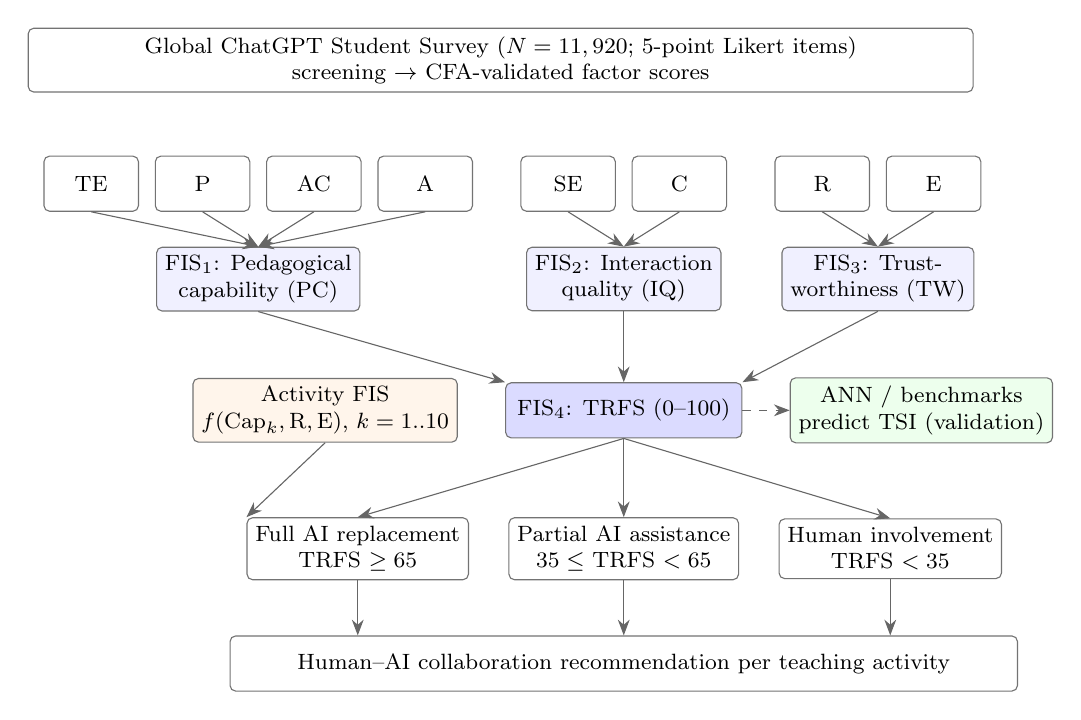
\begin{tikzpicture}[
  node distance=4mm and 6mm,
  box/.style={draw=black!55, rounded corners=2pt, align=center, font=\footnotesize, inner sep=3pt, minimum height=7mm, fill=white},
  fac/.style={box, minimum width=12mm},
  subsys/.style={box, fill=blue!6, minimum width=24mm},
  outbox/.style={box, fill=blue!14, minimum width=30mm},
  catbox/.style={box, minimum width=27mm},
  arr/.style={-{Stealth[length=2mm]}, draw=black!60}]
\node[box, minimum width=120mm] (data) {Global ChatGPT Student Survey ($N=\Nfinal$; 5-point Likert items)\\ screening $\rightarrow$ CFA-validated factor scores};
\node[fac, below=8mm of data.south west, anchor=north west, xshift=2mm] (te) {TE};
\node[fac, right=2mm of te] (p) {P};
\node[fac, right=2mm of p] (ac) {AC};
\node[fac, right=2mm of ac] (a) {A};
\node[fac, right=6mm of a] (se) {SE};
\node[fac, right=2mm of se] (c) {C};
\node[fac, right=6mm of c] (r) {R};
\node[fac, right=2mm of r] (e) {E};
\node[subsys, below=8mm of $(p)!0.5!(ac)$] (pc) {FIS$_1$: Pedagogical\\capability (PC)};
\node[subsys, below=8mm of $(se)!0.5!(c)$] (iq) {FIS$_2$: Interaction\\quality (IQ)};
\node[subsys, below=8mm of $(r)!0.5!(e)$] (tw) {FIS$_3$: Trust-\\worthiness (TW)};
\node[outbox, below=9mm of iq] (trfs) {FIS$_4$: TRFS (0--100)};
\foreach \x in {te,p,ac,a} \draw[arr] (\x.south) -- (pc.north);
\foreach \x in {se,c} \draw[arr] (\x.south) -- (iq.north);
\foreach \x in {r,e} \draw[arr] (\x.south) -- (tw.north);
\draw[arr] (pc.south) -- (trfs.north west);
\draw[arr] (iq.south) -- (trfs.north);
\draw[arr] (tw.south) -- (trfs.north east);
\node[catbox, below=10mm of trfs] (part) {Partial AI assistance\\$35\le$ TRFS $<65$};
\node[catbox, left=5mm of part] (full) {Full AI replacement\\TRFS $\ge 65$};
\node[catbox, right=5mm of part] (hum) {Human involvement\\TRFS $<35$};
\draw[arr] (trfs.south) -- (full.north);
\draw[arr] (trfs.south) -- (part.north);
\draw[arr] (trfs.south) -- (hum.north);
\node[box, fill=orange!8, left=6mm of trfs, minimum width=30mm] (act) {Activity FIS\\$f(\text{Cap}_k,\mathrm{R},\mathrm{E})$, $k=1..10$};
\node[box, fill=green!7, right=6mm of trfs, minimum width=30mm] (ann) {ANN / benchmarks\\predict TSI (validation)};
\draw[arr] (act.south) -- (full.north west);
\draw[arr, dashed] (trfs.east) -- (ann.west);
\node[box, below=7mm of part, minimum width=100mm] (rec) {Human--AI collaboration recommendation per teaching activity};
\draw[arr] (full.south) -- (rec.north -| full.south);
\draw[arr] (part.south) -- (rec.north);
\draw[arr] (hum.south) -- (rec.north -| hum.south);
\end{tikzpicture}}
\caption{Soft-computing framework for assessing the feasibility of AI substitution of teaching activities. TE: teaching effectiveness; P: personalization; AC: assessment capability; A: adaptability; SE: student engagement; C: communication; R: reliability; E: ethical suitability; TSI: teacher substitution index.}
\label{fig:framework}
\end{figure}

\subsection{Mathematical properties of the framework}
\label{sec:math}
Before applying the framework we establish its formal properties. Let $\mathcal{P}=\{\mu_L,\mu_M,\mu_H\}$ denote a three-term partition of a universe $U$.

\begin{proposition}[Decision thresholds]
\label{prop:thresholds}
On the output universe $[0,100]$ the Low/Medium and Medium/High membership functions intersect at $y=35$ and $y=65$, and on the Likert universe at $x=2.5$ and $x=3.5$. These crossover points are the unique values at which a score is equally a member of two adjacent linguistic classes.
\end{proposition}
\begin{proof}
On $[20,50]$, $\mu_L(y)=(50-y)/30$ and $\mu_M(y)=(y-20)/30$; equating gives $y^\ast=35$. On $[50,80]$, $\mu_M(y)=(80-y)/30=\mu_H(y)=(y-50)/30$ gives $y^\ast=65$. Outside these intervals at most one of each pair is positive. The Likert case is identical with knots $(2,3,4)$.
\end{proof}

\begin{proposition}[Rule-base complexity]
\label{prop:complexity}
A flat three-term rule base over $n$ inputs requires $3^n$ rules. A two-level hierarchy that partitions the inputs into groups of sizes $n_1,\dots,n_m$ and aggregates the $m$ group outputs requires $\sum_{i=1}^{m}3^{n_i}+3^{m}$ rules. For the present design ($n=8$; $n_i=4,2,2$; $m=3$) this is $3^4+3^2+3^2+3^3=\HierRules$ instead of $3^8=\FlatRules$, a reduction of \RuleReduction\%.
\end{proposition}
\begin{proof}
Each complete sub-system with $k$ three-term inputs enumerates $3^k$ antecedent combinations; the total is the sum over the $m+1$ sub-systems.
\end{proof}

\paragraph{Consequent centroids} For a trapezoid $\mathrm{trap}(a,b,c,d)$ the centroid has the closed form
\begin{equation}
\bar y(a,b,c,d)=\frac{(c^2+cd+d^2)-(a^2+ab+b^2)}{3\,[(c+d)-(a+b)]},
\label{eq:centroid-closed}
\end{equation}
obtained by integrating $y\,\mu(y)$ over the two linear flanks and the plateau. For the output terms this gives $c_L=\bar y(0,0,20,50)=3900/210=\cLval$, $c_M=50$ and, by symmetry, $c_H=100-c_L=\cHval$. Numerical integration on a $2\times10^5$-point grid reproduces $c_L$ to three decimals (\cLnum).

\paragraph{A provably monotone inference variant} Policy use of a feasibility score requires that improving any input factor can never \emph{lower} the score. Mamdani min--max inference with centroid defuzzification does not guarantee this property. We therefore also define a weighted-average (WA) variant on the same partitions and rule tables, with product t-norm and consequent centroids $c_{\ell}$:
\begin{equation}
f(\mathbf{x})=\frac{\sum_{\boldsymbol{\ell}\in\{L,M,H\}^k}\big(\prod_{j=1}^{k}\mu_{\ell_j}(x_j)\big)\,c_{r(\boldsymbol{\ell})}}{\sum_{\boldsymbol{\ell}}\prod_{j=1}^{k}\mu_{\ell_j}(x_j)},
\label{eq:wa}
\end{equation}
where $r(\boldsymbol{\ell})$ is the consequent of rule $\boldsymbol{\ell}$.

\begin{lemma}
\label{lem:ruspini}
Both partitions are Ruspini partitions, i.e.\ $\sum_{\ell}\mu_\ell(x)=1$ for all $x\in U$. Consequently the denominator of Eq.~\eqref{eq:wa} equals one, and $f$ is the multilinear interpolation of the rule table on the knot grid.
\end{lemma}
\begin{proof}
On $[2,3]$ only $\mu_L=3-x$ and $\mu_M=x-2$ are positive and they sum to one; on $[3,4]$, $\mu_M+\mu_H=(4-x)+(x-3)=1$; on $[1,2]$ and $[4,5]$ a single shoulder equals one. The output partition is analogous with slopes $1/30$. The denominator factorises as $\prod_j\sum_{\ell}\mu_\ell(x_j)=1$.
\end{proof}

\begin{lemma}
\label{lem:monotone-table}
All five rule tables of the framework are monotone: the consequent level is non-decreasing in every antecedent level.
\end{lemma}
\begin{proof}
For the rounded-mean rules the consequent is $\lceil \mathbf{w}^\top\boldsymbol{\ell}/\mathbf{1}^\top\mathbf{w}-\tfrac12\rceil$ with $\mathbf{w}>0$, a composition of a non-decreasing linear form and the non-decreasing ceiling function. For the veto rules (FIS$_3$, FIS$_4$ and the activity FIS) the consequent is Low on the veto set and the rounded mean elsewhere; raising a vetoing input from Low either keeps the consequent at Low or moves it to a non-negative level, so monotonicity is preserved. Exhaustive enumeration of the 153 rules confirms this (Table~\ref{tab:math}).
\end{proof}

\begin{proposition}[Boundedness, continuity, monotonicity and Lipschitz continuity of the WA framework]
\label{prop:monotone}
Let each sub-system be evaluated by Eq.~\eqref{eq:wa}. Then (i) every sub-system output lies in $[c_L,c_H]=[\cLval,\cHval]$; (ii) every output is continuous; (iii) every output is non-decreasing in each of its inputs; (iv) the hierarchical TRFS is non-decreasing in each of the eight factors; and (v) on the Likert scale $|\partial f/\partial x_j|\le c_H-c_L$ wherever the derivative exists.
\end{proposition}
\begin{proof}
(i) By Lemma~\ref{lem:ruspini}, $f$ is a convex combination of values in $\{c_L,c_M,c_H\}$. (ii) $f$ is a finite sum of products of continuous functions. (iii) Fix all inputs except $x_j$ and write $f=\sum_{\ell}\mu_\ell(x_j)\,g(\ell)$ with $g(\ell)=\sum_{\boldsymbol{\ell}_{-j}}\prod_{i\ne j}\mu_{\ell_i}(x_i)\,c_{r(\ell,\boldsymbol{\ell}_{-j})}$. By Lemma~\ref{lem:monotone-table} and $c_L<c_M<c_H$, $g$ is a non-negative combination of non-decreasing sequences and is therefore non-decreasing in $\ell$. On $[2,3]$, $f=(3-x_j)g(L)+(x_j-2)g(M)$, so $\partial f/\partial x_j=g(M)-g(L)\ge0$; on $[3,4]$, $\partial f/\partial x_j=g(H)-g(M)\ge0$; on $[1,2]$ and $[4,5]$, $f$ is constant in $x_j$. Being continuous and piecewise non-decreasing, $f$ is non-decreasing. (iv) The TRFS is the composition $f_4(f_1,f_2,f_3)$ of non-decreasing functions whose intermediate values lie in the domain $[0,100]$ of $f_4$ by (i); compositions of non-decreasing functions are non-decreasing. (v) $|g(\ell+1)-g(\ell)|\le c_H-c_L$ because $g$ is a convex combination of values in $[c_L,c_H]$.
\end{proof}

\begin{remark}
\label{rem:mamdani}
The Mamdani system shares property (i) only approximately: its range is $[18.44,81.56]$ on the 201-point grid, essentially $[c_L,c_H]$. It violates (iii). An exhaustive grid search (Table~\ref{tab:math}) found local decreases of up to \MamWorst{} TRFS points in up to \MamShare\% of grid steps, caused by the non-additive max aggregation and the centroid operator. Fig.~\ref{fig:surf3d} visualises these ripples. We retain Mamdani inference as the primary specification, because it matches the original proposal and is the standard in educational fuzzy evaluation, and report the provably monotone WA variant as a robustness check and as the recommended choice for operational decision support.
\end{remark}

\begin{figure}[!htbp]
\centering
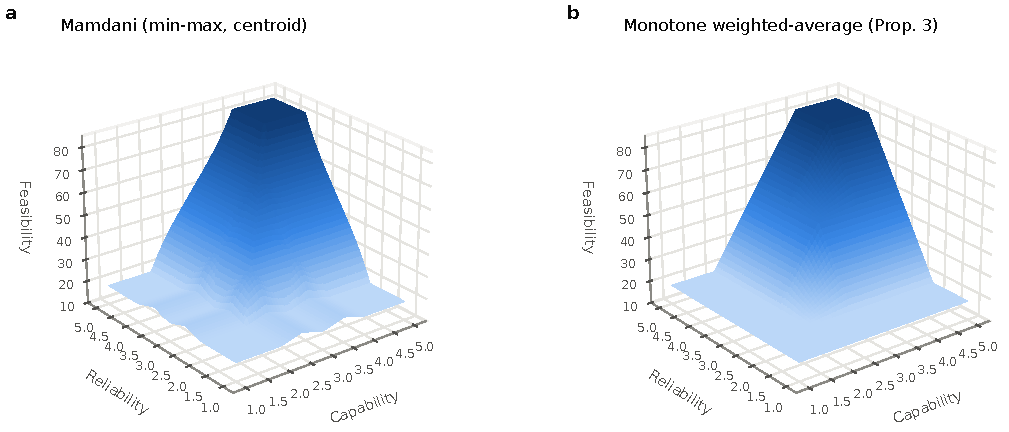
\includegraphics[width=\textwidth]{fig16_surfaces_3d.pdf}
\caption{Three-dimensional control surfaces of the activity FIS (ethical suitability fixed at 3): (a) Mamdani min--max inference with centroid defuzzification, showing local non-monotone ripples; (b) the weighted-average variant of Proposition~\ref{prop:monotone}, which is smooth and monotone by construction. Orange contours mark the 35 and 65 decision thresholds.}
\label{fig:surf3d}
\end{figure}

\begin{table}[!htbp]
\centering
\caption{Exhaustive grid verification of the mathematical properties. ``Worst decrease'' is the largest drop of the output between two adjacent grid points when one input increases; ``\% decreasing'' is the share of such steps. The weighted-average (WA) variant attains exactly $[c_L,c_H]$ and never decreases (differences are at floating-point precision), as guaranteed by Proposition~\ref{prop:monotone}.}
\label{tab:math}
\resizebox{\textwidth}{!}{%
\begin{tabular}{lcccccccc}
\toprule
 & & Monotone & Grid & \multicolumn{3}{c}{Mamdani (min--max, centroid)} & \multicolumn{2}{c}{Weighted average (product)}\\
\cmidrule(lr){5-7}\cmidrule(lr){8-9}
System & Rules & rule table & points & Range & Worst decrease & \% decreasing & Range & Worst decrease\\
\midrule
FIS$_1$ PC(TE,P,AC,A) & 81 & yes & 28,561 & [18.44, 81.56] & 1.85 & 0.9 & [18.57, 81.43] & $<10^{-13}$\\
FIS$_2$ IQ(SE,C) & 9 & yes & 1,681 & [18.44, 81.56] & 1.68 & 5.8 & [18.57, 81.43] & $<10^{-13}$\\
FIS$_3$ TW(R,E) & 9 & yes & 1,681 & [18.44, 81.56] & 1.68 & 8.5 & [18.57, 81.43] & $<10^{-13}$\\
FIS$_4$ TRFS(PC,IQ,TW) & 27 & yes & 68,921 & [18.44, 81.56] & 1.88 & 8.3 & [18.57, 81.43] & $<10^{-13}$\\
Activity FIS(Cap,R,E) & 27 & yes & 35,937 & [18.44, 81.56] & 2.70 & 9.4 & [18.57, 81.43] & $<10^{-13}$\\
\bottomrule
\end{tabular}}
\end{table}


%======================================================================
\section{Materials and methods}
\label{sec:methods}
%======================================================================

\subsection{Data source}
We used the open dataset \emph{Higher Education Students' Early Perceptions of ChatGPT: Global Survey Data} \citep{ravselj2024data}, released under a CC~BY~4.0 licence and described in \citet{ravselj2025}. The survey was coordinated by the University of Ljubljana with more than 200 international partners. It was administered online in seven languages between October 2023 and February 2024, using convenience sampling of students enrolled in higher education institutions. Participation was voluntary and anonymous, and respondents gave informed consent; the questionnaire is distributed with the dataset. It comprises eleven sections, including usage, perceived capabilities of ChatGPT, regulation and ethical concerns, satisfaction and attitude, study issues and outcomes, and skills development. Almost all items use five-point Likert scales (1~=~strongly disagree, 5~=~strongly agree). The released file contains \Ntotal{} responses and 174 variables. Because the study is a secondary analysis of fully anonymised open data, no additional ethical approval was required. Free-text institution names were removed from all derived files.

\subsection{Analytic sample}
Inclusion criteria were applied in sequence. (i) Respondents had to have used ChatGPT (Q13~=~yes; $n=\Nusers$), because questions on capabilities were shown only to users. (ii) Reported age had to be between 18 and 100 years ($n=\Nage$). (iii) Responses had to be complete on every item used in the models ($n=\Ncomplete$). (iv) Straight-liners, i.e.\ respondents giving the same answer to all model items, were excluded ($n=\Nstraight$ removed). The final analytic sample comprised $N=\Nfinal$ students (mean age \AgeMean, SD \AgeSD) studying in \Ncountries{} countries (Table~\ref{tab:demographics}). We used listwise deletion because the model items were presented as matrix blocks and missingness reflected survey break-off rather than item-level non-response.

\begin{table}[!htbp]
\centering
\caption{Profile of the analytic sample ($N=\Nfinal$ ChatGPT-using higher education students, \Ncountries{} countries of study).}
\label{tab:demographics}
\small
\begin{tabular}{lrr}
\toprule
Characteristic & $n$ & \% \\
\midrule
\multicolumn{3}{l}{\textit{Gender}}\\
\quad Male & 5,266 & 44.2\\
\quad Female & 6,476 & 54.3\\
\quad Other & 50 & 0.4\\
\quad Prefer not to say & 106 & 0.9\\
\multicolumn{3}{l}{\textit{Level of study}}\\
\quad Undergraduate & 9,856 & 82.7\\
\quad Postgraduate (Master) & 1,455 & 12.2\\
\quad Doctoral & 516 & 4.3\\
\multicolumn{3}{l}{\textit{Field of study}}\\
\quad Arts \& Humanities & 1,423 & 11.9\\
\quad Social Sciences & 4,824 & 40.5\\
\quad Applied Sciences & 4,274 & 35.9\\
\quad Natural \& Life Sciences & 1,291 & 10.8\\
\multicolumn{3}{l}{\textit{Mode of study}}\\
\quad Traditional & 5,450 & 45.7\\
\quad Online & 1,015 & 8.5\\
\quad Blended & 5,389 & 45.2\\
\multicolumn{3}{l}{\textit{ChatGPT version used}}\\
\quad ChatGPT-3.5 (free) & 10,550 & 88.5\\
\quad ChatGPT-4 (paid) & 384 & 3.2\\
\quad Both & 958 & 8.0\\
\bottomrule
\end{tabular}
\end{table}


\subsection{Operationalisation}
\paragraph{Evaluation factors} Each of the eight factors of the original framework was measured by three to five questionnaire items describing ChatGPT's performance on that dimension (Table~\ref{tab:measurement}). Ethical suitability (E) was measured by five concern items (e.g.\ ``ChatGPT might encourage students to cheat''), reverse-coded so that higher scores indicate fewer ethical concerns. Factor scores are item means on the 1--5 scale. An initial \emph{a priori} mapping showed poor discriminant validity (HTMT~$>1$) and low reliability for two factors. We therefore compared four candidate mappings on CFA fit, AVE and HTMT and retained the best-fitting, theoretically coherent one. All candidates and their fit statistics are reported in the replication package (\texttt{measurement\_alternatives.csv}).

\paragraph{Teaching activities} The ten activities listed in the original proposal were each operationalised by the items in which students rate ChatGPT on that activity (Table~\ref{tab:activities}). Examples are ``simplify complex information'' and ``summarize extensive information'' for \emph{content explanation}, ``improve my readiness for exams'' and ``improve my grades'' for \emph{student assessment}, and ``improve my problem-solving / analytical / critical-thinking skills'' for \emph{problem solving}. For \emph{emotional and social support} we combined interpersonal-communication and pleasant-conversation items with reverse-coded concerns that ChatGPT might reduce human interaction or increase social isolation.

\paragraph{Independent criterion} To validate the fuzzy score and to train the ANN we needed an outcome that was not used as a fuzzy input. We constructed a \emph{Teacher Substitution Index} (TSI) from the only two items that compare ChatGPT directly with professors: ``It is easier for me to interact with ChatGPT than with my professors'' (Q24b) and ``The information I get from ChatGPT is clearer than the one provided by my professors'' (Q24d). The TSI is their mean, rescaled to 0--100.

\subsection{Measurement validation}
Internal consistency was assessed with Cronbach's $\alpha$ \citep{cronbach1951} and composite reliability (CR). We estimated a correlated eight-factor confirmatory factor analysis (CFA) by maximum likelihood on the item correlation matrix, with each item loading on one factor and latent variances fixed to one. Global fit was evaluated with CFI, TLI, RMSEA and SRMR against conventional cut-offs \citep{hu1999,kline2016}. Convergent validity was assessed through standardised loadings and the average variance extracted (AVE), and discriminant validity through the Fornell--Larcker criterion \citep{fornell1981} and the heterotrait--monotrait ratio (HTMT; threshold 0.85, \citealp{henseler2015}). Because all variables come from one self-report instrument, common-method variance was screened with Harman's single-factor test \citep{podsakoff2003}.

\subsection{Hierarchical fuzzy inference system}
\paragraph{Fuzzification} Each input factor $x\in[1,5]$ is described by three linguistic terms with trapezoidal and triangular membership functions (Fig.~\ref{fig:mf}a):
\begin{equation}
\begin{aligned}
\mu_{\text{Low}}(x)&=\mathrm{trap}(x;1,1,2,3),\qquad
\mu_{\text{Med}}(x)=\mathrm{tri}(x;2,3,4),\\
\mu_{\text{High}}(x)&=\mathrm{trap}(x;3,4,5,5),
\end{aligned}
\end{equation}
so that the Likert anchors 1--2, 3 and 4--5 are full members of Low, Medium and High respectively. The intermediate variables (PC, IQ, TW) and the output TRFS live on $[0,100]$ with
\begin{equation}
\begin{aligned}
\mu_{\text{Low}}(y)&=\mathrm{trap}(y;0,0,20,50),\qquad
\mu_{\text{Med}}(y)=\mathrm{tri}(y;20,50,80),\\
\mu_{\text{High}}(y)&=\mathrm{trap}(y;50,80,100,100)
\end{aligned}
\end{equation}
(Fig.~\ref{fig:mf}b).

\begin{figure}[!htbp]
\centering
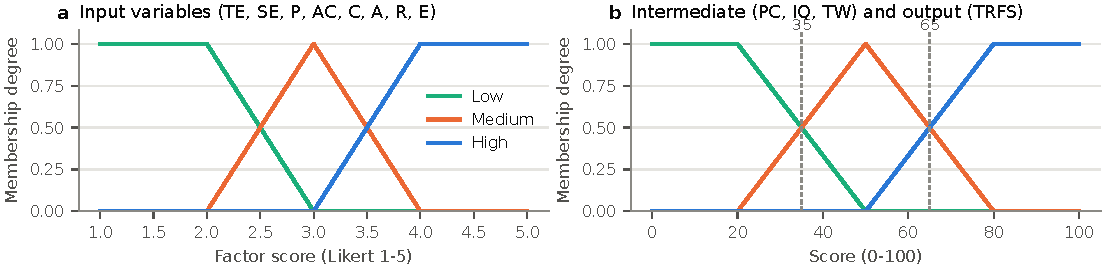
\includegraphics[width=\textwidth]{fig2_membership_functions.pdf}
\caption{Membership functions of (a) the eight input factors and (b) the intermediate and output variables. Dashed lines mark the Low/Medium (35) and Medium/High (65) crossover points used as decision thresholds.}
\label{fig:mf}
\end{figure}

\paragraph{Rule bases} The rules encode the logic of the original proposal in a systematic, reproducible form. For PC and IQ, the consequent is the rounded mean of the antecedent levels (Low~$=0$, Medium~$=1$, High~$=2$), with ties resolved conservatively towards the lower class. This yields 81 and 9 rules. Trustworthiness implements a reliability veto (``IF reliability is low THEN feasibility is low''); ethical suitability then moderates the result (Table~\ref{tab:rules}). The final system FIS$_4$ gives pedagogical capability double weight, $\ell=(2\,\ell_{\mathrm{PC}}+\ell_{\mathrm{IQ}}+\ell_{\mathrm{TW}})/4$, and applies the trust veto (TW Low $\Rightarrow$ TRFS Low). For example, PC High, IQ Low and TW Medium gives Medium, which corresponds to Rule~2 of the original proposal (``high teaching effectiveness BUT low communication $\Rightarrow$ medium'').

\begin{table}[!htbp]
\centering
\caption{Rule bases of the trust sub-system FIS$_3$ (top) and the final system FIS$_4$ (bottom; L/M/H = Low/Medium/High).}
\label{tab:rules}
\footnotesize
\begin{tabular}{lccc}
\toprule
FIS$_3$: TW & E = Low & E = Medium & E = High\\
\midrule
R = Low & Low & Low & Low\\
R = Medium & Low & Medium & Medium\\
R = High & Medium & High & High\\
\bottomrule
\end{tabular}

\vspace{0.6em}
\setlength{\tabcolsep}{3pt}
\begin{tabular}{rcccc|rcccc|rcccc}
\toprule
\# & PC & IQ & TW & TRFS & \# & PC & IQ & TW & TRFS & \# & PC & IQ & TW & TRFS\\
\midrule
1 & L & L & L & L & 10 & M & L & L & L & 19 & H & L & L & L\\
2 & L & L & M & L & 11 & M & L & M & M & 20 & H & L & M & M\\
3 & L & L & H & L & 12 & M & L & H & M & 21 & H & L & H & M\\
4 & L & M & L & L & 13 & M & M & L & L & 22 & H & M & L & L\\
5 & L & M & M & L & 14 & M & M & M & M & 23 & H & M & M & M\\
6 & L & M & H & M & 15 & M & M & H & M & 24 & H & M & H & H\\
7 & L & H & L & L & 16 & M & H & L & L & 25 & H & H & L & L\\
8 & L & H & M & M & 17 & M & H & M & M & 26 & H & H & M & H\\
9 & L & H & H & M & 18 & M & H & H & M & 27 & H & H & H & H\\
\bottomrule
\end{tabular}
\end{table}


\paragraph{Inference and defuzzification} For a respondent with inputs $\mathbf{x}$, the firing strength of rule $r$ is $w_r=\min_j \mu_{A_{rj}}(x_j)$. The aggregated output set is $\mu(y)=\max_r \min\{w_r,\mu_{B_r}(y)\}$, and the crisp output is its centroid
\begin{equation}
\mathrm{TRFS}=\frac{\int_0^{100} y\,\mu(y)\,dy}{\int_0^{100}\mu(y)\,dy},
\label{eq:centroid}
\end{equation}
evaluated on a 201-point grid \citep{mamdani1975,ross2010}. The intermediate outputs of FIS$_{1\text{--}3}$ are fed to FIS$_4$ as crisp values. The system is implemented in vectorised NumPy; scoring all respondents takes less than one second.

\paragraph{Decision categories} The crossover points of the output terms define the three categories of the original proposal: \emph{full AI replacement} (TRFS~$\ge 65$), \emph{partial AI assistance} ($35\le$~TRFS~$<65$) and \emph{human involvement required} (TRFS~$<35$). The thresholds were fixed before the data were analysed.

\subsection{Activity-level fuzzy system}
For activity $k$ we define $\mathrm{Cap}_k$ as the mean of its items. The activity FIS computes $\mathrm{TRFS}_k=f(\mathrm{Cap}_k,\mathrm{R},\mathrm{E})$ with the same membership functions. Its 27 rules mirror the proposal (Rule~1: capability and reliability High $\Rightarrow$ High; Rule~3: capability or reliability Low $\Rightarrow$ Low). Otherwise the consequent is the weighted level mean $(2\ell_{\mathrm{Cap}}+\ell_{\mathrm{R}}+\ell_{\mathrm{E}})/4$. Each activity is classified by its mean score; we also report the share of respondents in each category and bootstrap 95\% confidence intervals (2000 resamples; \citealp{efron1993}). Differences between activities were tested with the Friedman test \citep{friedman1937}, with Kendall's $W$ as effect size. Adjacent activities in the ranking were compared with Wilcoxon signed-rank tests, using Holm-adjusted $p$-values \citep{holm1979} and the matched-pairs rank-biserial correlation as effect size.

\subsection{Neural network and benchmark models}
The ANN is a multilayer perceptron \citep{rumelhart1986} that maps the eight standardised factors to the TSI. It uses ReLU activations, Adam optimisation \citep{kingma2015}, mini-batches of 128, early stopping on a 15\% validation split and L2 regularisation. Architecture (one hidden layer of 16 units, or two hidden layers of 32--16 or 64--32 units) and penalty ($\alpha\in\{10^{-4},10^{-2}\}$) were tuned by an inner 3-fold grid search within every outer training fold. This nested design keeps tuning separate from evaluation. We compared the ANN with:
(a) a \emph{hybrid fuzzy--ANN}, the same tuned MLP with the HFIS outputs (PC, IQ, TW, TRFS) as four additional inputs;
(b) ordinary least-squares \emph{linear regression};
(c) \emph{support vector regression} with an RBF kernel \citep{smola2004};
(d) \emph{random forest} \citep{breiman2001};
(e) \emph{gradient boosting} \citep{friedman2001}; and
(f) the \emph{calibrated fuzzy score}, a one-parameter linear rescaling of the TRFS fitted on each training fold, which uses no other information from the TSI.
All models were evaluated by \CVsplits-fold cross-validation repeated \CVrepeats{} times (\CVfits{} train/test splits) using MSE, RMSE, MAE and $R^2$. Because fold scores from repeated cross-validation are not independent, model differences were tested with the corrected resampled $t$-test of \citet{nadeau2003}. To check whether the network can represent the expert system itself, we also trained an MLP to reproduce the TRFS from the eight factors (5-fold cross-validated fidelity).

\subsection{Factor importance}
RQ2 was examined from three complementary angles: (i) Spearman correlations of each factor with the TSI; (ii) permutation importance of the ANN, i.e.\ the drop in out-of-fold $R^2$ when a factor is randomly permuted (5 folds $\times$ 10 repeats); and (iii) the local sensitivity of the HFIS, i.e.\ the mean change in TRFS when a factor is increased by one standard deviation for every respondent.

\subsection{Robustness analysis}
Every fuzzy system depends on design choices. To test how much the activity ranking and classification depend on them, we drew \RobDraws{} random configurations. Each draw shifted the input membership functions by $U(-0.25,0.25)$ Likert points and changed their spread by $U(-0.25,0.25)$; shifted the output sets by $U(-5,5)$ points and changed their spread by $U(-5,5)$; switched the tie-breaking rule (conservative vs.\ liberal rounding); and switched the t-norm (minimum vs.\ product). For each draw we recorded Kendall's $\tau$ between the perturbed and the baseline activity ranking and the share of activities that kept their category.

\subsection{Extended statistical analyses}
\label{sec:extended-methods}
\paragraph{Shapley decomposition of explained variance} To apportion the explained variance of the TSI among correlated factors without the order dependence of sequential $R^2$, we computed the Shapley value of each factor in the cooperative game whose characteristic function is the OLS coefficient of determination \citep{lipovetsky2001}. This is equivalent to the general dominance weights of \citet{budescu1993}:
\begin{equation}
\phi_j=\sum_{S\subseteq P\setminus\{j\}}\frac{|S|!\,(p-|S|-1)!}{p!}\Big[R^2(S\cup\{j\})-R^2(S)\Big],\qquad R^2(S)=\mathbf{r}_S^{\top}\mathbf{R}_{SS}^{-1}\mathbf{r}_S,
\label{eq:shapley}
\end{equation}
where $\mathbf{R}$ is the factor correlation matrix and $\mathbf{r}$ the vector of factor--TSI correlations. By the efficiency axiom, $\sum_j\phi_j=R^2(P)$ exactly. All $2^8=256$ subset models were evaluated, and 95\% CIs were obtained from \ShapB{} bootstrap resamples.

\paragraph{Multilevel modelling} Students are nested in countries. We fitted random-intercept models $y_{ic}=\mathbf{x}_{ic}^{\top}\boldsymbol\beta+u_c+\varepsilon_{ic}$ with $u_c\sim\mathcal N(0,\tau^2)$ and $\varepsilon_{ic}\sim\mathcal N(0,\sigma^2)$ by REML \citep{raudenbush2002} for the \MlCountries{} countries with at least \MlMinN{} respondents ($n=\MlN$). We report the intraclass correlation $\mathrm{ICC}=\tau^2/(\tau^2+\sigma^2)$, the marginal and conditional $R^2$ of \citet{nakagawa2013}, $R^2_m=\sigma_f^2/(\sigma_f^2+\tau^2+\sigma^2)$ and $R^2_c=(\sigma_f^2+\tau^2)/(\sigma_f^2+\tau^2+\sigma^2)$, and a likelihood-ratio test of $\tau^2=0$. The test uses the boundary-corrected reference distribution $\tfrac12\chi^2_0+\tfrac12\chi^2_1$ \citep{self1987}. Country effects are shown as best linear unbiased predictors with conditional standard errors $\sqrt{\tau^2\sigma^2/(n_c\tau^2+\sigma^2)}$.

\paragraph{Quantile regression} To test whether the TRFS--TSI relationship is homogeneous across the criterion distribution, we estimated $Q_{\tau}(\mathrm{TSI}\mid\mathrm{TRFS})=\beta_0(\tau)+\beta_1(\tau)\,\mathrm{TRFS}/10$ for $\tau=0.10,\dots,0.90$ by minimising $\sum_i\rho_\tau(y_i-\mathbf{x}_i^{\top}\boldsymbol\beta)$ with $\rho_\tau(u)=u\,(\tau-\mathbb 1\{u<0\})$ \citep{koenker1978}. The TSI takes only nine values, so we applied the jittering approach of \citet{machado2005}: we added $U(-6.25,6.25)$ noise (half the TSI step) and averaged the estimates over \QReps{} replications.

\paragraph{Effect sizes and equivalence tests} For each activity we computed Cohen's $d_z=(\bar x-50)/s$ against the neutral centre of the partial-assistance band, with $\mathrm{SE}(d_z)\approx\sqrt{1/n+d_z^2/(2n)}$. Because the large sample makes almost every difference ``significant'', we also tested \emph{practical equivalence} to 50 with the two one-sided tests (TOST) procedure \citep{schuirmann1987,lakens2017}. The smallest effect size of interest was $\Delta=\pm\TostDelta$ TRFS points (2\% of the scale). Equivalence is declared when both $t_1=(\bar x-(50-\Delta))/\mathrm{SE}$ and $t_2=(\bar x-(50+\Delta))/\mathrm{SE}$ reject their one-sided nulls at $\alpha=0.05$.

\paragraph{Measurement invariance} We fitted the eight-factor CFA separately by gender, level of study, field of study and questionnaire language (groups with $n\ge300$). For each factor we compared group loadings $\boldsymbol\lambda_g$ with pooled loadings $\boldsymbol\lambda_0$ using Tucker's congruence coefficient
\begin{equation}
\varphi(\boldsymbol\lambda_g,\boldsymbol\lambda_0)=\frac{\sum_i\lambda_{gi}\lambda_{0i}}{\sqrt{\sum_i\lambda_{gi}^2\sum_i\lambda_{0i}^2}},
\label{eq:tucker}
\end{equation}
where $\varphi\ge0.95$ indicates that the factors can be considered equal \citep{lorenzo2006}.

\paragraph{Student typologies} To identify groups of students with similar activity-capability profiles we applied $k$-means clustering \citep{lloyd1982} to the ten standardised activity capabilities for $k=2,\dots,6$. The number of clusters was fixed by a pre-declared rule: the highest mean silhouette $s(i)=(b_i-a_i)/\max(a_i,b_i)$ \citep{rousseeuw1987} among solutions whose bootstrap stability, the mean adjusted Rand index \citep{hubert1985} over 20 resamples, was at least 0.90. Distributions of all activity scores are visualised as raincloud plots \citep{allen2019}.

\subsection{Subgroup analysis and software}
Differences in TRFS by gender, level of study, field of study, mode of study and ChatGPT version were tested with Kruskal--Wallis tests, with $\varepsilon^2$ as effect size. All analyses were run in Python~3.13 with NumPy, pandas, SciPy and scikit-learn \citep{pedregosa2011}. The CFA was estimated with a purpose-written maximum-likelihood routine (SciPy L-BFGS-B). A fixed random seed (2024) was used throughout. The complete pipeline, which regenerates every table and figure, is available in the replication package (see Data and code availability). All analysis tables that are not shown in the main text are reported in Appendix~\ref{app:tables}.

%======================================================================
\section{Results}
\label{sec:results}
%======================================================================

\subsection{Measurement model}
The eight-factor CFA fitted the data acceptably: $\chi^2(\CfaDf)=\ChiSq$ (significant, as expected with $N>10{,}000$), CFI~$=\CFIval$, TLI~$=\TLIval$, RMSEA~$=\RMSEAval$, SRMR~$=\SRMRval$. RMSEA and SRMR meet the stricter cut-offs of \citet{hu1999}, and CFI/TLI exceed the conventional 0.90 benchmark. All standardised loadings were at least \LoadMin. Cronbach's $\alpha$ and CR exceeded 0.70 for every factor (Table~\ref{tab:measurement}). AVE was at or above 0.50 for six factors and marginally below it for student engagement and communication. For these two factors CR~$>0.70$ still indicates adequate convergent validity \citep{fornell1981}. All HTMT ratios were below 0.85 (maximum \HTMTmax; Table~\ref{tab:htmt}), supporting discriminant validity. The stricter Fornell--Larcker criterion was not met for the three learning-outcome factors (SE, P and AC), whose latent correlations reached 0.79; we return to this in Section~\ref{sec:limitations}. Harman's first factor explained \Harman\% of the item variance, well below 50\%, so common-method variance is unlikely to dominate the results.

\begin{table}[!htbp]
\centering
\caption{Operationalisation of the eight evaluation factors and measurement-model results (standardised CFA loadings $\lambda$, Cronbach's $\alpha$, composite reliability CR, average variance extracted AVE). Items marked (R) are reverse-coded. CFA fit: $\chi^2(\CfaDf)=\ChiSq$, CFI~$=\CFIval$, TLI~$=\TLIval$, RMSEA~$=\RMSEAval$, SRMR~$=\SRMRval$.}
\label{tab:measurement}
\footnotesize
\resizebox{\textwidth}{!}{%
\begin{tabular}{p{2.7cm}lp{7.4cm}cccc}
\toprule
Factor & Item & Wording (abridged) & $\lambda$ & $\alpha$ & CR & AVE \\
\midrule
\multirow{3}{*}{\parbox{2.6cm}{Teaching effectiveness (TE)}} & Q19d & ChatGPT can provide information efficiently & 0.647 & \multirow{3}{*}{0.741} & \multirow{3}{*}{0.750} & \multirow{3}{*}{0.501}\\
 & Q19f & ChatGPT can summarize extensive information & 0.730 & & &\\
 & Q19g & ChatGPT can simplify complex information & 0.742 & & &\\
\midrule
\multirow{3}{*}{\parbox{2.6cm}{Student engagement (SE)}} & Q25b & Using ChatGPT is interesting to me & 0.676 & \multirow{3}{*}{0.742} & \multirow{3}{*}{0.746} & \multirow{3}{*}{0.495}\\
 & Q25c & Being able to use ChatGPT is important to me & 0.747 & & &\\
 & Q25d & ChatGPT can help with things in everyday life & 0.685 & & &\\
\midrule
\multirow{3}{*}{\parbox{2.6cm}{Personalization (P)}} & Q26d & ChatGPT can provide me with personalized education & 0.707 & \multirow{3}{*}{0.772} & \multirow{3}{*}{0.779} & \multirow{3}{*}{0.541}\\
 & Q26a & ChatGPT can enhance my access to sources of knowledge & 0.712 & & &\\
 & Q26c & ChatGPT can improve my specific knowledge & 0.786 & & &\\
\midrule
\multirow{3}{*}{\parbox{2.6cm}{Assessment capability (AC)}} & Q27a & ChatGPT can improve my readiness for exams & 0.795 & \multirow{3}{*}{0.817} & \multirow{3}{*}{0.819} & \multirow{3}{*}{0.602}\\
 & Q27b & ChatGPT can improve my grades & 0.789 & & &\\
 & Q26j & ChatGPT can improve the quality of my assignments & 0.743 & & &\\
\midrule
\multirow{3}{*}{\parbox{2.6cm}{Communication (C)}} & Q19a & ChatGPT can understand indications given in human language & 0.743 & \multirow{3}{*}{0.714} & \multirow{3}{*}{0.734} & \multirow{3}{*}{0.484}\\
 & Q19b & ChatGPT can respond in human language & 0.769 & & &\\
 & Q19c & ChatGPT can hold a pleasant conversation & 0.554 & & &\\
\midrule
\multirow{3}{*}{\parbox{2.6cm}{Adaptability (A)}} & Q19h & ChatGPT can facilitate traditional (classroom) learning & 0.719 & \multirow{3}{*}{0.858} & \multirow{3}{*}{0.864} & \multirow{3}{*}{0.682}\\
 & Q19i & ChatGPT can facilitate online learning & 0.866 & & &\\
 & Q19j & ChatGPT can facilitate blended (hybrid) learning & 0.882 & & &\\
\midrule
\multirow{3}{*}{\parbox{2.6cm}{Reliability (R)}} & Q19e & ChatGPT can provide reliable information & 0.610 & \multirow{3}{*}{0.813} & \multirow{3}{*}{0.827} & \multirow{3}{*}{0.619}\\
 & Q24f & Satisfied with the quality of information provided & 0.867 & & &\\
 & Q24g & Satisfied with the accuracy of information provided & 0.857 & & &\\
\midrule
\multirow{5}{*}{\parbox{2.6cm}{Ethical suitability (E)}} & Q22a & ChatGPT might encourage unethical behaviour (R) & 0.647 & \multirow{5}{*}{0.867} & \multirow{5}{*}{0.870} & \multirow{5}{*}{0.579}\\
 & Q22b & ChatGPT might encourage students to cheat (R) & 0.882 & & &\\
 & Q22c & ChatGPT might encourage students to plagiarize (R) & 0.877 & & &\\
 & Q22d & ChatGPT might threaten the ethics of the study (R) & 0.800 & & &\\
 & Q22f & ChatGPT might invade privacy (R) & 0.538 & & &\\
\bottomrule
\end{tabular}}
\end{table}

\begin{table}[!htbp]
\centering
\caption{Discriminant validity. Lower triangle: HTMT ratios; diagonal (bold): $\sqrt{\mathrm{AVE}}$; upper triangle (italic): latent CFA correlations.}
\label{tab:htmt}
\footnotesize
\setlength{\tabcolsep}{3.5pt}
\begin{tabular}{lcccccccc}
\toprule
 & TE & SE & P & AC & C & A & R & E\\
\midrule
TE & \textbf{0.71} & \textit{0.49} & \textit{0.54} & \textit{0.49} & \textit{0.60} & \textit{0.58} & \textit{0.55} & \textit{0.09}\\
SE & 0.51 & \textbf{0.70} & \textit{0.75} & \textit{0.71} & \textit{0.44} & \textit{0.52} & \textit{0.52} & \textit{0.18}\\
P & 0.55 & 0.76 & \textbf{0.74} & \textit{0.79} & \textit{0.40} & \textit{0.53} & \textit{0.61} & \textit{0.18}\\
AC & 0.51 & 0.72 & 0.81 & \textbf{0.78} & \textit{0.36} & \textit{0.55} & \textit{0.55} & \textit{0.19}\\
C & 0.65 & 0.49 & 0.45 & 0.40 & \textbf{0.70} & \textit{0.43} & \textit{0.36} & \textit{0.04}\\
A & 0.60 & 0.53 & 0.55 & 0.56 & 0.47 & \textbf{0.83} & \textit{0.43} & \textit{0.14}\\
R & 0.67 & 0.51 & 0.64 & 0.57 & 0.43 & 0.49 & \textbf{0.79} & \textit{0.17}\\
E & 0.13 & 0.20 & 0.20 & 0.21 & 0.09 & 0.16 & 0.20 & \textbf{0.76}\\
\bottomrule
\end{tabular}
\end{table}


\subsection{Factor profile}
Students rated ChatGPT's teaching effectiveness highest (Fig.~\ref{fig:profile}a). This factor captures summarising, simplifying and efficiently providing information. Student engagement, personalization and communication followed. Reliability and ethical suitability received the lowest scores, close to the scale midpoint. The latent correlations (Fig.~\ref{fig:profile}b) show a tight cluster of learning-outcome factors (SE, P, AC). Ethical suitability was almost unrelated to perceived capability ($r\le\PhiEmax$): students who consider ChatGPT capable do not necessarily consider it ethically unproblematic.

\begin{figure}[!htbp]
\centering
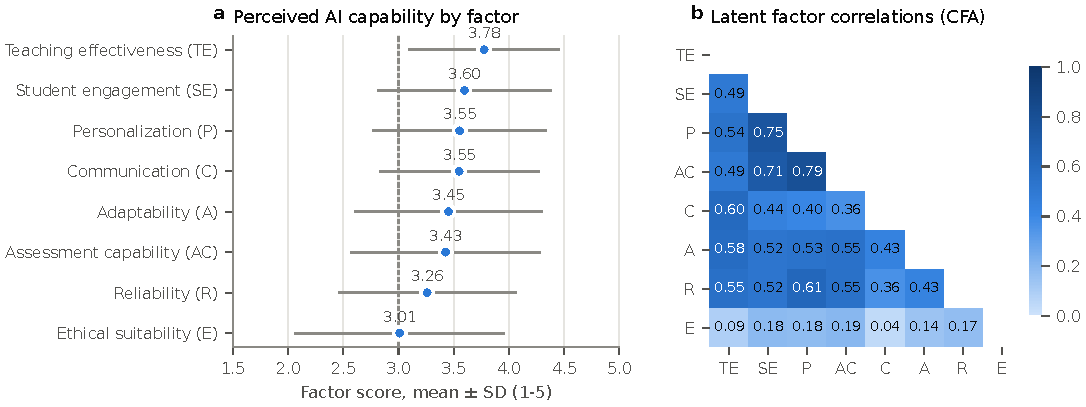
\includegraphics[width=\textwidth]{fig4_factor_profile.pdf}
\caption{(a) Mean ($\pm$ SD) scores of the eight evaluation factors; the dashed line marks the neutral midpoint. (b) Latent factor correlations from the CFA.}
\label{fig:profile}
\end{figure}

\subsection{Overall feasibility score and its validity (RQ3)}
The mean overall TRFS was \TRFSmean{} (SD~\TRFSsd, median \TRFSmedian). The first-level outputs were \PCmean{} for pedagogical capability, \IQmean{} for interaction quality and \TWmean{} for trustworthiness: students credit AI with considerable pedagogical capability but only moderate trustworthiness. At the respondent level, \PctFull\% of students fell into the full-replacement band, \PctPartial\% into partial assistance and \PctHuman\% into human involvement (Fig.~\ref{fig:trfs}a). The multimodal distribution is a known property of centroid defuzzification with few output terms: respondents whose inputs fire the same rules receive similar crisp scores.

The fuzzy score behaved as a valid measure (Fig.~\ref{fig:trfs}b). Although no TSI information entered the fuzzy system, the TRFS correlated positively with the TSI ($\rho=\RhoTSI$). It also correlated with satisfaction with ChatGPT's assistance ($\rho=\RhoSat$), overall experience ($\rho=\RhoExp$) and intensity of use ($\rho=\RhoUse$; Kruskal--Wallis $H=\KWusageH$, $p<0.001$). It was unrelated to the concern that ChatGPT ``might replace formal education'' ($\rho=\RhoReplace$, $p=\PReplace$). This discriminant result shows that the TRFS captures perceived task capability rather than general anxiety about AI displacing education.

\begin{figure}[!htbp]
\centering
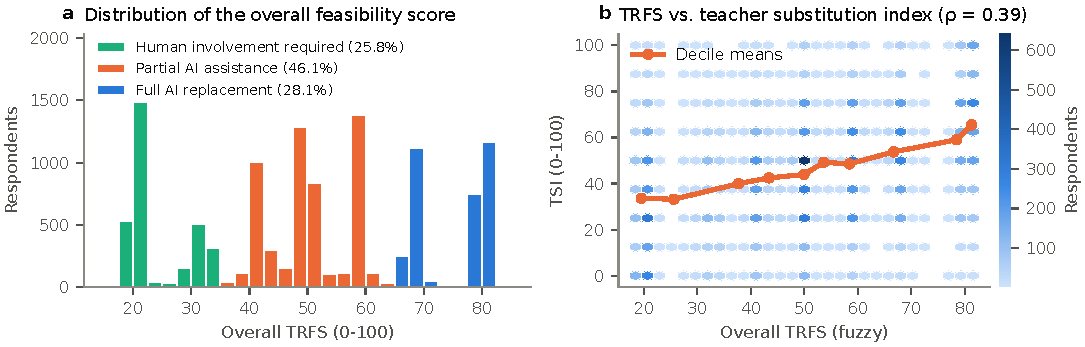
\includegraphics[width=\textwidth]{fig5_trfs_distribution_validity.pdf}
\caption{(a) Distribution of the overall TRFS, coloured by decision category. (b) TRFS against the independent Teacher Substitution Index; points are binned (hexagons) and the line connects TRFS-decile means.}
\label{fig:trfs}
\end{figure}

\subsection{Feasibility of individual teaching activities (RQ1, RQ4)}
Table~\ref{tab:activities} and Fig.~\ref{fig:activities} present the activity-level results. Activities differed significantly (Friedman $\chi^2(9)=\FriedmanChi$, $p<0.001$). The effect was small (Kendall's $W=\KendallW$), so the differences are systematic but modest compared with the variation between students. After Holm correction all adjacent pairs in the ranking differed significantly. The only exception in substance is classroom communication versus emotional and social support, whose mean difference was negligible (0.01 points, rank-biserial $r=-0.04$); these two activities are effectively tied.

\emph{Content explanation} (\act{A1}{score}, 95\% CI [\act{A1}{lo}, \act{A1}{hi}]) and \emph{question answering} (\act{A2}{score}) ranked highest. For these two activities the share of students placing AI in the full-replacement band (\act{A1}{full}\% and \act{A2}{full}\%) clearly exceeded the share requiring human involvement (\act{A1}{human}\% and \act{A2}{human}\%). \emph{Personalized learning} (\act{A5}{score}) also lay reliably above the neutral centre. \emph{Assignment feedback} (\act{A3}{score}) was balanced. \emph{Student assessment}, \emph{student motivation}, \emph{academic guidance}, \emph{emotional and social support}, \emph{classroom communication} and \emph{problem solving} lay reliably below the neutral centre. Problem solving ranked lowest (\act{A9}{score}) and had the largest human-involvement share (\act{A9}{human}\%).

The central result for RQ4 is that \emph{no activity reached the full-replacement band}: all ten mean scores fall in the partial-assistance range (35--65). Within this range, the bootstrap confidence intervals separate an \emph{AI-leaning} group (explanation, question answering, personalised learning) from a \emph{human-leaning} group (assessment, motivation, guidance, socio-emotional support, classroom communication and higher-order problem solving).

\begin{table}[!htbp]
\centering
\caption{Activity-level Teacher Replacement Feasibility Scores. Capability is the mean of the activity's items (1--5); TRFS is the mean activity-FIS output with a bootstrap 95\% CI (2000 resamples); the next three columns give the share of respondents whose individual score falls in each decision category (Full $\geq$ 65, Partial 35--65, Human $<$ 35). All ten activity means fall in the \emph{Partial AI assistance} band; the tier indicates whether the CI lies above, across or below the neutral centre (50) of that band.}
\label{tab:activities}
\footnotesize
\setlength{\tabcolsep}{4pt}
\resizebox{\textwidth}{!}{%
\begin{tabular}{rllccccccl}
\toprule
Rank & Teaching activity & Items & Capability & TRFS [95\% CI] & \% Full & \% Partial & \% Human & Tier \\
\midrule
1 & Content explanation (A1) & Q19g, Q19f, Q26b & 3.80 & 54.7 [54.3, 55.0] & 31.6 & 52.0 & 16.3 & AI-leaning\\
2 & Question answering (A2) & Q19a, Q19b, Q19d & 3.65 & 53.3 [52.9, 53.6] & 28.7 & 53.5 & 17.9 & AI-leaning\\
3 & Personalized learning (A5) & Q26d, Q26e & 3.46 & 50.9 [50.6, 51.3] & 22.2 & 57.3 & 20.4 & AI-leaning\\
4 & Assignment feedback (A3) & Q26j, Q28a, Q28b & 3.42 & 50.3 [49.9, 50.6] & 24.1 & 52.0 & 23.9 & Balanced\\
5 & Student assessment (A4) & Q27a, Q27b & 3.36 & 49.4 [49.0, 49.7] & 20.3 & 56.1 & 23.6 & Human-leaning\\
6 & Student motivation (A6) & Q26f, Q27i & 3.32 & 49.1 [48.7, 49.4] & 20.1 & 55.9 & 24.0 & Human-leaning\\
7 & Academic guidance (A8) & Q27h, Q27g, Q27j & 3.27 & 48.6 [48.2, 48.9] & 21.7 & 51.6 & 26.7 & Human-leaning\\
8 & Emotional \& social support (A10) & Q28f, Q19c, Q22g, Q22i & 3.18 & 48.1 [47.8, 48.5] & 16.5 & 60.5 & 23.1 & Human-leaning\\
9 & Classroom communication (A7) & Q19h, Q26h & 3.23 & 48.1 [47.8, 48.5] & 16.1 & 60.4 & 23.5 & Human-leaning\\
10 & Problem solving (A9) & Q29c, Q29d, Q29e & 3.14 & 46.5 [46.2, 46.9] & 19.0 & 49.9 & 31.1 & Human-leaning\\
\bottomrule
\end{tabular}}
\end{table}


\begin{figure}[!htbp]
\centering
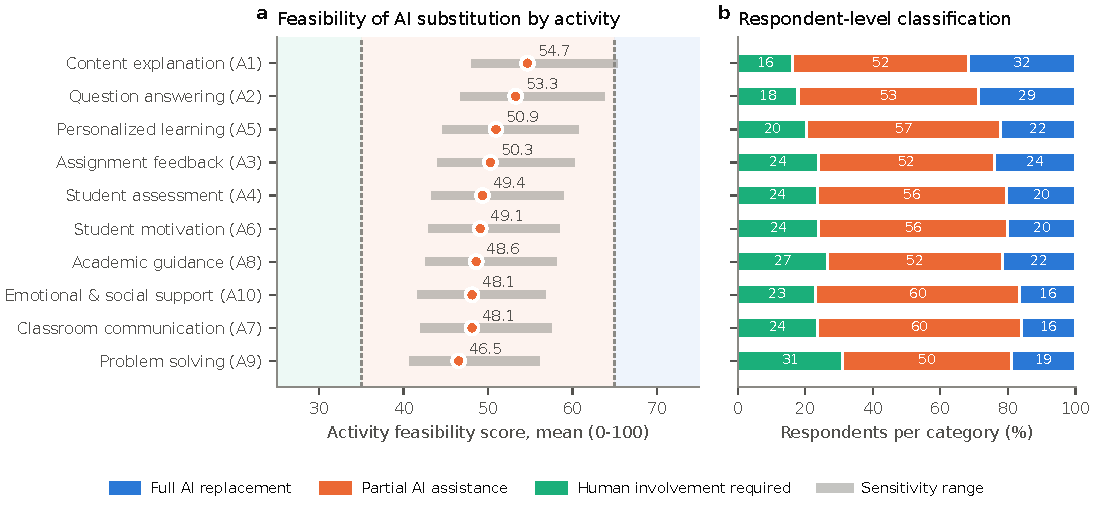
\includegraphics[width=\textwidth]{fig8_activity_feasibility.pdf}
\caption{(a) Mean activity feasibility scores. Grey bars show the 2.5--97.5\% range across \RobDraws{} perturbed fuzzy designs; shaded bands mark the decision categories. (b) Share of respondents in each decision category per activity.}
\label{fig:activities}
\end{figure}

\subsection{Fuzzy versus neural modelling (RQ3)}
Table~\ref{tab:models} and Fig.~\ref{fig:models} compare the predictive models. The tuned ANN achieved the lowest error (RMSE~$=\AnnRMSE$, $R^2=\AnnRsq$); the configuration selected most often by the inner grid search had two hidden layers of 64 and 32 units with $\alpha=10^{-2}$. Gradient boosting performed identically ($R^2=\GbRsq$, $p\GbP$), and random forest was not significantly worse ($R^2=\RfRsq$, $p\RfP$). The ANN was significantly more accurate than linear regression ($R^2=\LrRsq$, $p\LrP$) and SVR ($R^2=\SvrRsq$, $p\SvrP$), but the gain over the linear model was below one percentage point of explained variance. The factor--criterion relationships are therefore mildly non-linear but dominated by additive linear effects. Supplying the fuzzy intermediate outputs to the network did not help: the hybrid fuzzy--ANN was slightly but significantly worse than the plain ANN ($R^2=\HybRsq$, $p\HybP$), presumably because the four extra inputs are deterministic functions of the original eight and add variance to the tuning process without adding information. The calibrated fuzzy score, which was not trained on the TSI at all, reached $R^2=\FisRsq$. This is significantly lower than the ANN ($p\FisP$) but still \FisShare\% of the ANN's explained variance, obtained from \emph{a priori} rules that can be read in full. The modest absolute $R^2$ values are typical for single-occasion attitude data and indicate that perceived AI capability is one of several determinants of students' willingness to substitute AI for their professors. Finally, an MLP reproduced the fuzzy system almost perfectly from the eight factors (cross-validated $R^2=\SurrRsq$, RMSE~$=\SurrRMSE$), so the HFIS mapping can also be learned by a network.

\begin{table}[!htbp]
\centering
\caption{Out-of-fold prediction of the Teacher Substitution Index (TSI, 0--100) from the eight factors: mean (SD) over \CVsplits-fold cross-validation repeated \CVrepeats{} times (\CVfits{} folds). $t$ and $p$: Nadeau--Bengio corrected resampled $t$-test on fold RMSE against the ANN. The calibrated fuzzy model uses no TSI information except a one-parameter linear rescaling of the TRFS fitted on each training fold.}
\label{tab:models}
\footnotesize
\resizebox{\textwidth}{!}{%
\begin{tabular}{lcccccc}
\toprule
Model & MSE & RMSE & MAE & $R^2$ & $t$ vs ANN & $p$ \\
\midrule
\textbf{ANN (MLP)} & 467.3 (15.2) & 21.61 (0.35) & 17.39 (0.37) & 0.259 (0.023) & -- & --\\
Gradient boosting & 467.3 (15.6) & 21.62 (0.36) & 17.32 (0.36) & 0.259 (0.022) & -0.03 & 0.975\\
Hybrid fuzzy-ANN & 469.8 (14.7) & 21.67 (0.34) & 17.45 (0.36) & 0.255 (0.022) & -2.64 & 0.013\\
Random forest & 469.8 (15.9) & 21.67 (0.37) & 17.33 (0.37) & 0.255 (0.023) & -1.30 & 0.204\\
Linear regression & 471.8 (15.9) & 21.72 (0.37) & 17.53 (0.38) & 0.252 (0.023) & -3.22 & 0.003\\
SVR (RBF) & 478.0 (16.0) & 21.86 (0.37) & 17.33 (0.35) & 0.242 (0.027) & -5.48 & $<$0.001\\
Fuzzy HFIS (calibrated) & 533.6 (19.2) & 23.10 (0.42) & 18.70 (0.39) & 0.155 (0.021) & -16.38 & $<$0.001\\
\bottomrule
\end{tabular}}
\end{table}


\begin{figure}[!htbp]
\centering
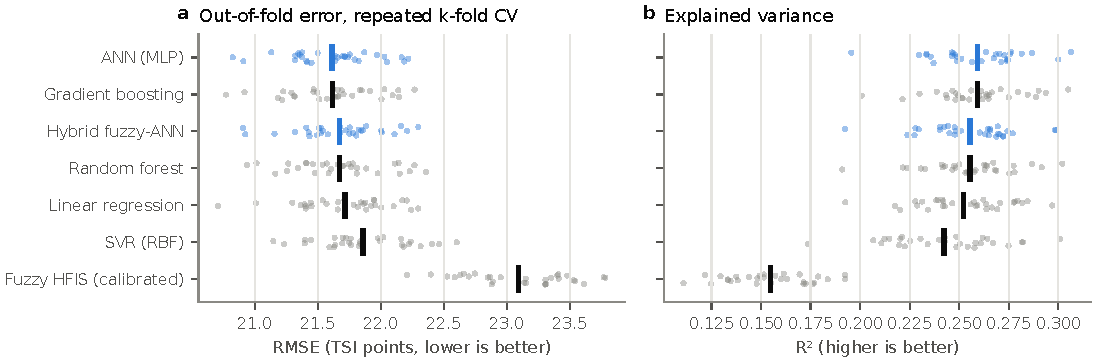
\includegraphics[width=\textwidth]{fig6_model_comparison.pdf}
\caption{Out-of-fold (a) RMSE and (b) $R^2$ for the TSI over \CVfits{} cross-validation folds (dots) and their means (vertical bars). The ANN variants are highlighted.}
\label{fig:models}
\end{figure}

\subsection{Determinants of feasibility (RQ2)}
Reliability was the most influential factor in both views (Table~\ref{tab:importance}, Fig.~\ref{fig:importance}). In the ANN, permuting reliability reduced $R^2$ by \ImpR. Assessment capability (\ImpAC), personalization (\ImpP) and student engagement (\ImpSE) followed. Teaching effectiveness, adaptability, ethical suitability and communication added little \emph{unique} predictive information once the other factors were known. This reflects their correlation with the remaining factors rather than irrelevance: teaching effectiveness, for example, correlated $\rho=\RhoTE$ with the TSI. In the fuzzy system, reliability was likewise the strongest lever (+1~SD raised TRFS by \SensR{} points). Ethical suitability came second (\SensE), because the rule base treats low trust as a veto. The two importance rankings agreed only moderately (Kendall's $\tau=\ImpTau$). The main disagreement concerns ethics: the expert-designed rules weight it heavily, whereas students' substitution judgements are almost unrelated to it ($\rho=\RhoE$). We discuss this normative--empirical gap below.

\begin{table}[!htbp]
\centering
\caption{Factor importance. $\rho$: Spearman correlation with TSI. ANN: mean (SD) drop in out-of-fold $R^2$ when the factor is permuted (5 folds $\times$ 10 permutations). FIS: mean change in TRFS when the factor is raised by one SD.}
\label{tab:importance}
\footnotesize
\setlength{\tabcolsep}{3.5pt}
\begin{tabular}{lccccc}
\toprule
Factor & $\rho$ & ANN $\Delta R^2$ & Rank & FIS $\Delta$TRFS & Rank \\
\midrule
Reliability (R) & 0.36 & 0.094 (0.004) & 1 & 6.46 & 1\\
Assessment capability (AC) & 0.40 & 0.075 (0.006) & 2 & 1.31 & 3\\
Student engagement (SE) & 0.35 & 0.045 (0.005) & 3 & 0.67 & 7\\
Personalization (P) & 0.39 & 0.045 (0.008) & 4 & 1.04 & 5\\
Teaching effectiveness (TE) & 0.20 & 0.020 (0.003) & 5 & 0.58 & 8\\
Adaptability (A) & 0.28 & 0.016 (0.004) & 6 & 1.20 & 4\\
Ethical suitability (E) & 0.09 & 0.008 (0.002) & 7 & 3.49 & 2\\
Communication (C) & 0.16 & 0.003 (0.002) & 8 & 0.98 & 6\\
\bottomrule
\end{tabular}
\end{table}


\begin{figure}[!htbp]
\centering
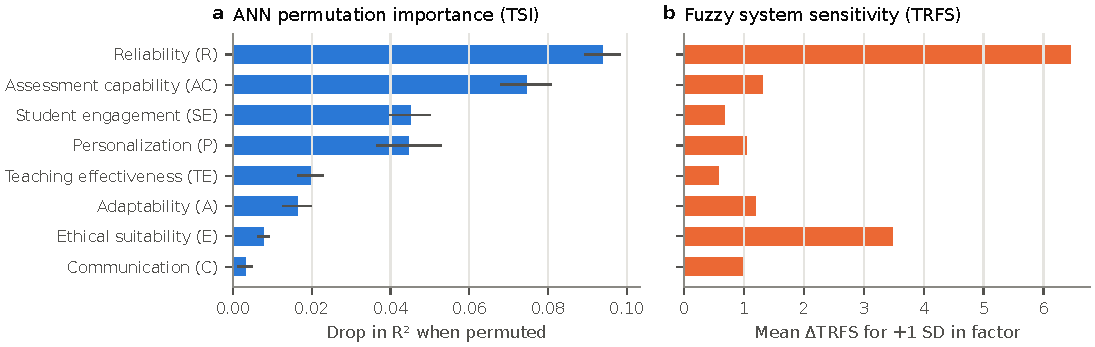
\includegraphics[width=\textwidth]{fig7_factor_importance.pdf}
\caption{Factor importance: (a) permutation importance in the ANN predicting the TSI; (b) sensitivity of the fuzzy TRFS to a one-SD increase in each factor.}
\label{fig:importance}
\end{figure}

\subsection{Robustness and subgroups}
The activity ranking was highly stable under perturbation of the fuzzy design. Across \RobDraws{} random configurations the mean Kendall's $\tau$ with the baseline ranking was \RobTau{} (5th percentile \RobTauLow), and on average \RobAgree\% of activities kept their category (minimum \RobAgreeMin\%; Fig.~\ref{fig:robust}). The perturbation ranges are shown as grey bars in Fig.~\ref{fig:activities}a. The conclusion that no activity reaches full replacement under the baseline design therefore does not hinge on fine details of the membership functions. Category changes occurred in only 3.4\% of the configurations (one or two activities each time). The central 95\% of perturbed activity scores lay between 40.8 and 65.3, so the changes occur at the upper boundary: content explanation was the only activity whose 97.5th percentile exceeded 65 (65.3). Question answering came close (63.8). These two activities are therefore the strongest candidates for AI-led delivery as capabilities improve.

Subgroup differences in the overall TRFS were statistically significant but negligible in size (all $\varepsilon^2\le\EpsMax$). The largest was by ChatGPT version: users of the paid version rated feasibility higher ($\varepsilon^2=\EpsVersion$). The activity ranking was almost identical across fields of study (Fig.~\ref{fig:field}), which suggests that the task-level pattern is a general feature of students' perceptions rather than a disciplinary artefact.

\begin{figure}[!htbp]
\centering
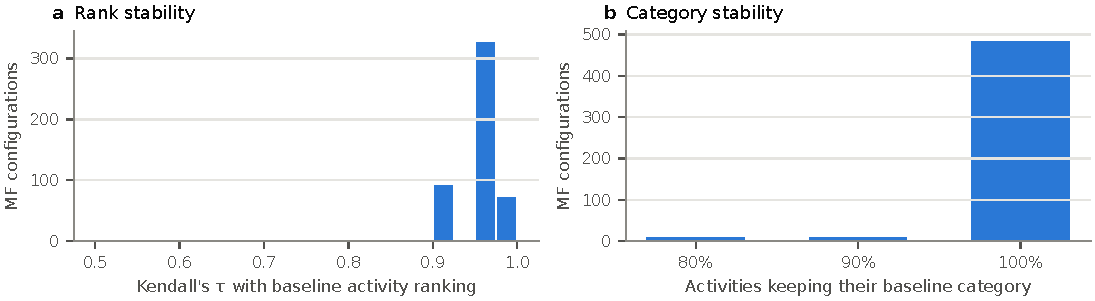
\includegraphics[width=\textwidth]{fig9_robustness.pdf}
\caption{Robustness of the activity-level results to \RobDraws{} random fuzzy designs: (a) rank agreement with the baseline; (b) share of activities keeping their baseline category.}
\label{fig:robust}
\end{figure}

\begin{figure}[!htbp]
\centering
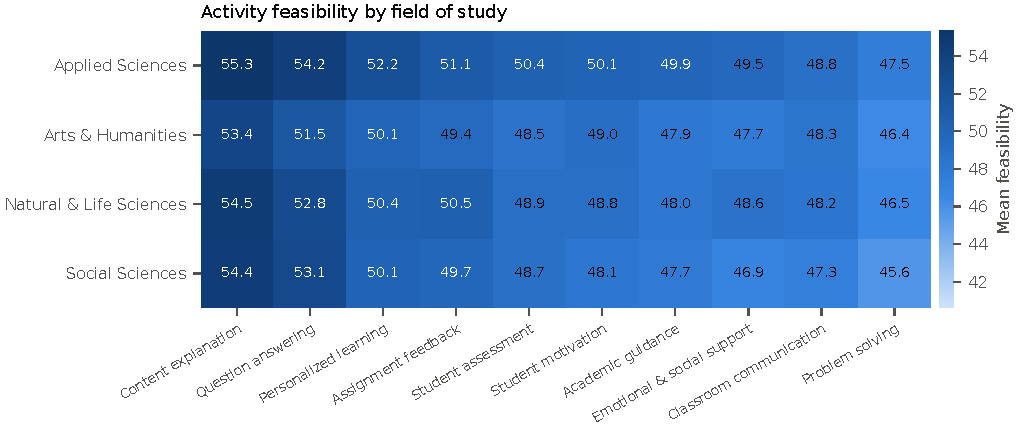
\includegraphics[width=\textwidth]{fig10_activity_by_field.pdf}
\caption{Mean activity feasibility scores by field of study (columns ordered by the overall ranking).}
\label{fig:field}
\end{figure}

\subsection{Mathematical verification}
The exhaustive grid checks in Table~\ref{tab:math} confirm Propositions~\ref{prop:thresholds}--\ref{prop:monotone} numerically. All rule tables are monotone, and the WA variant attains exactly $[\cLval,\cHval]$ without a single decreasing step. The Mamdani system shows the ripples described in Remark~\ref{rem:mamdani}. On the real data the two inference variants agreed closely: the overall scores correlated at $r=\RMamWa$ (Spearman $\rho=\RhoMamWa$), the WA score had a mean of \WaMean{} (SD~\WaSD), and its validity against the TSI was practically unchanged ($\rho=\RhoWaTSI$ vs.\ \RhoTSI). The activity ranking was almost identical (Kendall's $\tau=\WaTau$; Fig.~\ref{fig:effects}b). Under WA inference all ten activities again fell in the partial-assistance band (\WaMin--\WaMax). The substantive conclusions therefore do not depend on the choice between the conventional and the provably monotone inference scheme.

\subsection{Exact decomposition of explained variance}
The eight factors jointly explained $R^2=\ShapRsq$ of the TSI in OLS, and the Shapley values sum exactly to this total (Table~\ref{tab:shapley}, Fig.~\ref{fig:shapley}). Assessment capability carried the largest share (\ShapPctAC\%), followed by reliability (\ShapPctR\%), personalization (\ShapPctP\%) and student engagement (\ShapPctSE\%). Together these four account for more than 85\% of the explained variance. Ethical suitability contributed only \ShapPctE\%. The Shapley ranking differs from the ANN permutation ranking mainly in the order of the top two factors (AC vs.\ R): permutation importance measures \emph{unique} information, whereas Shapley values share overlapping variance fairly among correlated predictors.

\begin{figure}[!htbp]
\centering
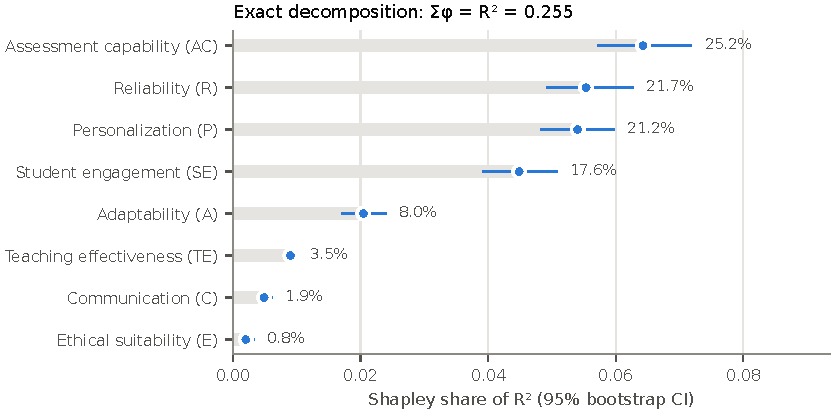
\includegraphics[width=0.75\textwidth]{fig12_shapley_r2.pdf}
\caption{Shapley decomposition of the explained variance of the TSI (Eq.~\ref{eq:shapley}); bars show $\phi_j$ with 95\% bootstrap CIs and labels the share of the total $R^2$.}
\label{fig:shapley}
\end{figure}

\begin{table}[!htbp]
\centering
\caption{Relative importance and multilevel effects of the eight factors on the TSI. Shapley values $\phi_j$ (Eq.~\ref{eq:shapley}) with 95\% bootstrap CIs (\ShapB{} resamples) sum exactly to $R^2=\ShapRsq$. $\beta$: fixed effect per +1~SD in a random-intercept model with students nested in \MlCountries{} countries ($n=\MlN$); OLS: single-level estimate for comparison.}
\label{tab:shapley}
\resizebox{\textwidth}{!}{%
\begin{tabular}{lccccc}
\toprule
Factor & Shapley $\phi_j$ [95\% CI] & \% of $R^2$ & Multilevel $\beta$ [95\% CI] & $p$ & OLS $\beta$\\
\midrule
Assessment capability (AC) & 0.0643 [0.0571, 0.0720] & 25.2 & 4.65 [4.10, 5.20] & $<$0.001 & 4.75\\
Reliability (R) & 0.0554 [0.0491, 0.0628] & 21.7 & 4.38 [3.86, 4.89] & $<$0.001 & 5.20\\
Personalization (P) & 0.0540 [0.0483, 0.0598] & 21.2 & 2.98 [2.41, 3.54] & $<$0.001 & 3.32\\
Student engagement (SE) & 0.0449 [0.0392, 0.0508] & 17.6 & 3.65 [3.13, 4.17] & $<$0.001 & 3.23\\
Adaptability (A) & 0.0204 [0.0170, 0.0240] & 8.0 & 1.49 [1.00, 1.99] & $<$0.001 & 1.48\\
Teaching effectiveness (TE) & 0.0090 [0.0082, 0.0100] & 3.5 & -1.94 [-2.46, -1.43] & $<$0.001 & -2.40\\
Communication (C) & 0.0049 [0.0041, 0.0062] & 1.9 & -0.49 [-0.95, -0.03] & 0.039 & -0.65\\
Ethical suitability (E) & 0.0020 [0.0013, 0.0033] & 0.8 & -0.02 [-0.43, 0.38] & 0.910 & -0.14\\
\midrule
\multicolumn{6}{l}{ICC (null model): TSI \IccTSI, TRFS \IccTRFS; marginal / conditional $R^2$ = \RsqMarg{} / \RsqCond; LR test for the country intercept: $\chi^2=\LRval$, $p<0.001$.}\\
\bottomrule
\end{tabular}}
\end{table}


\subsection{Country-level variation}
Country membership accounted for \IccTRFS{} of the variance of the TRFS and \IccTSI{} of the variance of the TSI (null-model ICCs). This variance is small but highly significant (LR~$=\LRval$, $p<0.001$). After the eight factors were controlled, the residual country ICC of the TSI fell to \IccCond. The fixed effects were very close to the single-level estimates (Fig.~\ref{fig:multilevel}b). Assessment capability ($\beta=\BetaAC$ TSI points per SD), reliability (\BetaR), student engagement (\BetaSE) and personalization (\BetaP) had the largest positive effects. Teaching effectiveness ($\beta=\BetaTE$) and communication (\BetaC) had small \emph{negative} conditional effects, a classic suppression pattern. Holding perceived learning benefits constant, students who mainly value ChatGPT for summarising and explaining are slightly \emph{less} inclined to see it as a substitute for their professors. Ethical suitability had no effect (\BetaE). The marginal and conditional $R^2$ were \RsqMarg{} and \RsqCond. Country mean TRFS ranged from about 40 to 71 (Fig.~\ref{fig:multilevel}a): it was highest in Estonia and in several African and Asian countries (e.g.\ Egypt, Ghana, Bangladesh and Tanzania) and lowest in, for example, Japan and Austria. National context therefore shifts the \emph{level} of perceived feasibility, but not the pattern of its determinants.

\begin{figure}[!htbp]
\centering
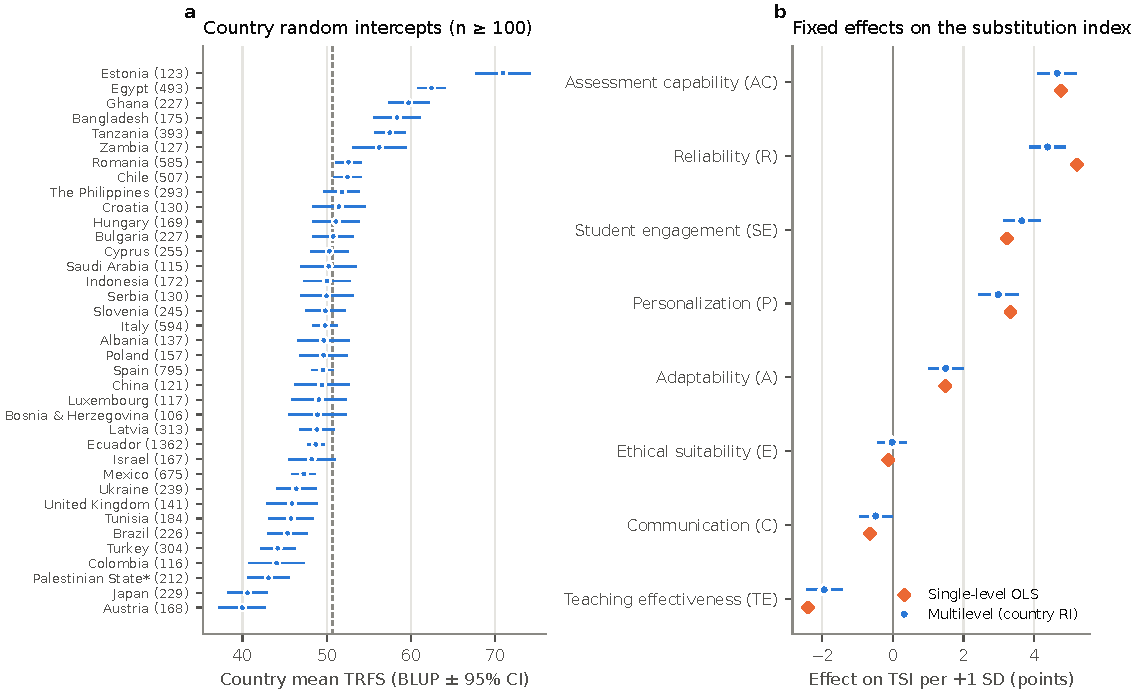
\includegraphics[width=\textwidth]{fig13_multilevel.pdf}
\caption{Multilevel results. (a) Country random intercepts for the TRFS (countries with $n\ge100$; BLUP $\pm$ 95\% CI; dashed line: grand mean). (b) Fixed effects of the eight standardised factors on the TSI from the random-intercept model, compared with single-level OLS.}
\label{fig:multilevel}
\end{figure}

\subsection{Heterogeneity across the criterion distribution and across students}
Quantile regression showed a positive TRFS effect at every quantile (Fig.~\ref{fig:quantile}). The effect was largest around the median ($\beta_{0.5}=\QbetaFifty$ TSI points per 10 TRFS points) and smaller in the tails ($\beta_{0.1}=\QbetaTen$, $\beta_{0.9}=\QbetaNinety$; OLS \QolsBeta). Perceived feasibility therefore discriminates best among students with moderate substitution attitudes. At the extremes, attitudes appear anchored by factors outside the framework.

\begin{figure}[!htbp]
\centering
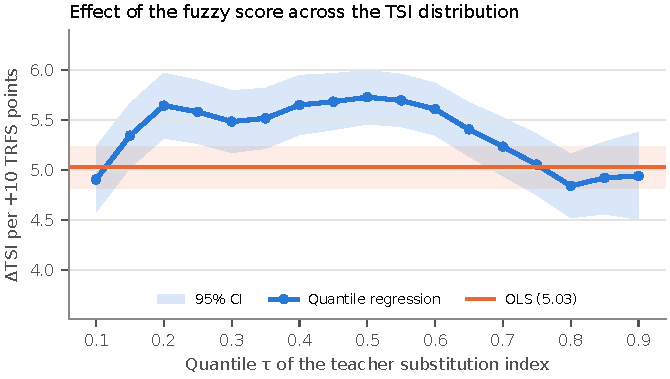
\includegraphics[width=0.75\textwidth]{fig14_quantile_regression.pdf}
\caption{Quantile-regression coefficients of the TSI on the TRFS (per 10 points) with 95\% CIs, averaged over \QReps{} jittered replications; the horizontal line and band show the OLS estimate and its CI.}
\label{fig:quantile}
\end{figure}

The selection rule retained $k=\TyK$ clusters (silhouette \SilTwo, bootstrap ARI \AriTwo). These separated an \emph{AI-sceptical} group (\TyPctScepTwo\%; mean TRFS \TyTrfsScepTwo) from an \emph{AI-receptive} group (\TyPctRecTwo\%; mean TRFS \TyTrfsRecTwo). The first principal component of the ten activity capabilities explained \TyPC\% of their variance. Students therefore differ mainly in their \emph{overall} level of confidence in AI and much less in the \emph{shape} of their profiles. The finer three-cluster solution (silhouette \SilThree, ARI \AriThree; Fig.~\ref{fig:typology}) is informative for policy. It distinguishes \emph{AI-sceptical} (\TyPctScepThree\%, TRFS \TyTrfsScepThree), \emph{ambivalent} (\TyPctAmbThree\%, TRFS \TyTrfsAmbThree) and \emph{AI-enthusiastic} students (\TyPctEnthThree\%, TRFS \TyTrfsEnthThree). For the enthusiastic third of students the mean overall score lies \emph{above} the full-replacement threshold. Two activities exceed 65 in this group (content explanation 66.0 and personalised learning 65.2), and most others lie just below it (Fig.~\ref{fig:typology}b). For the sceptical sixth, eight of the ten activities fall into the human-involvement band; only content explanation and question answering (both about 39) remain in the partial band. Content explanation is among the two highest-rated activities in every group, and problem solving is among the three lowest. The middle of the ranking differs between groups: sceptics, for example, place emotional and social support third, whereas enthusiasts place it last. This activity partly reflects concerns about reduced human contact (reverse-coded), which vary less with general AI confidence than the capability items do. Typology was only weakly associated with field of study (Cram\'er's $V=\TyVThree$), but it was clearly associated with the TSI ($\varepsilon^2=\TyEpsThree$).

\begin{figure}[!htbp]
\centering
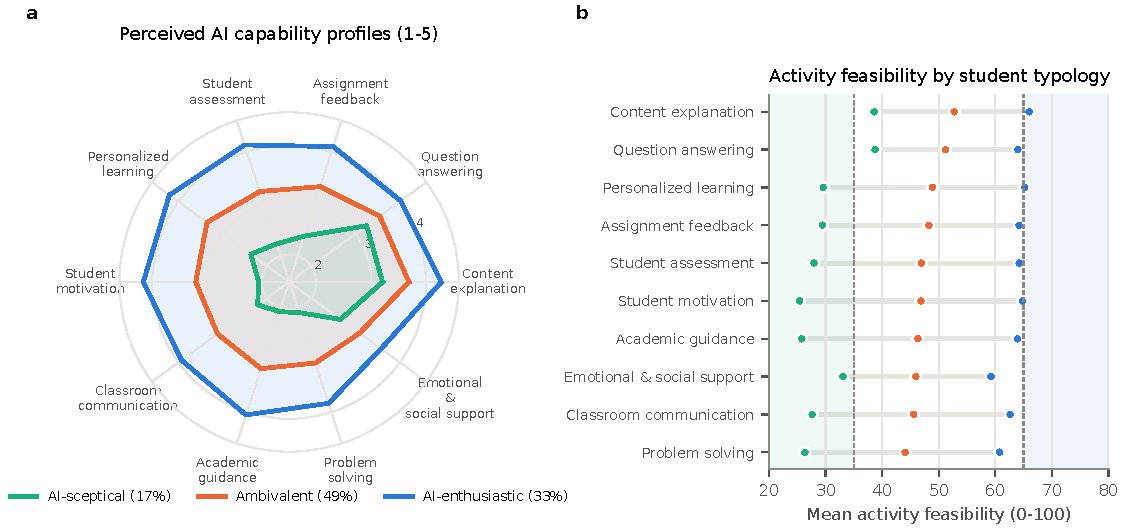
\includegraphics[width=\textwidth]{fig15_typology.pdf}
\caption{Student typologies ($k$-means, three-cluster solution). (a) Mean perceived capability per activity (1--5). (b) Mean activity feasibility scores per typology; shaded bands mark the human-involvement and full-replacement regions.}
\label{fig:typology}
\end{figure}

\subsection{Effect sizes, practical equivalence and measurement invariance}
Fig.~\ref{fig:raincloud} shows the full distribution of every activity score. The effect sizes against the neutral centre were small (Cohen's $d_z$ from \Dmin{} to \Dmax; Fig.~\ref{fig:effects}a). TOST established practical equivalence to 50 ($\pm\TostDelta$ points) for \TostN{} activities: personalised learning, assignment feedback, assessment, motivation and academic guidance. Their mean scores are thus statistically indistinguishable from a perfectly balanced human--AI split. Content explanation and question answering lay reliably above this band, and problem solving, classroom communication and socio-emotional support lay below it. Every activity mean was significantly below the 65-point replacement threshold (one-sided $p<0.001$).

The eight-factor model fitted acceptably in all \InvGroups{} subgroups (CFI~$\ge\InvCFI$, RMSEA~$\le\InvRMSEA$; Table~\ref{tab:invariance}). Tucker's congruence between group-specific and pooled loadings was at least \InvCong{} for every factor and group, well above the 0.95 criterion for factorial equality. The largest loading difference (\InvDiff) occurred in the smallest language groups. The factor scores therefore measure the same constructs across genders, levels, disciplines and questionnaire languages, and subgroup comparisons of the TRFS are meaningful.

\begin{figure}[!htbp]
\centering
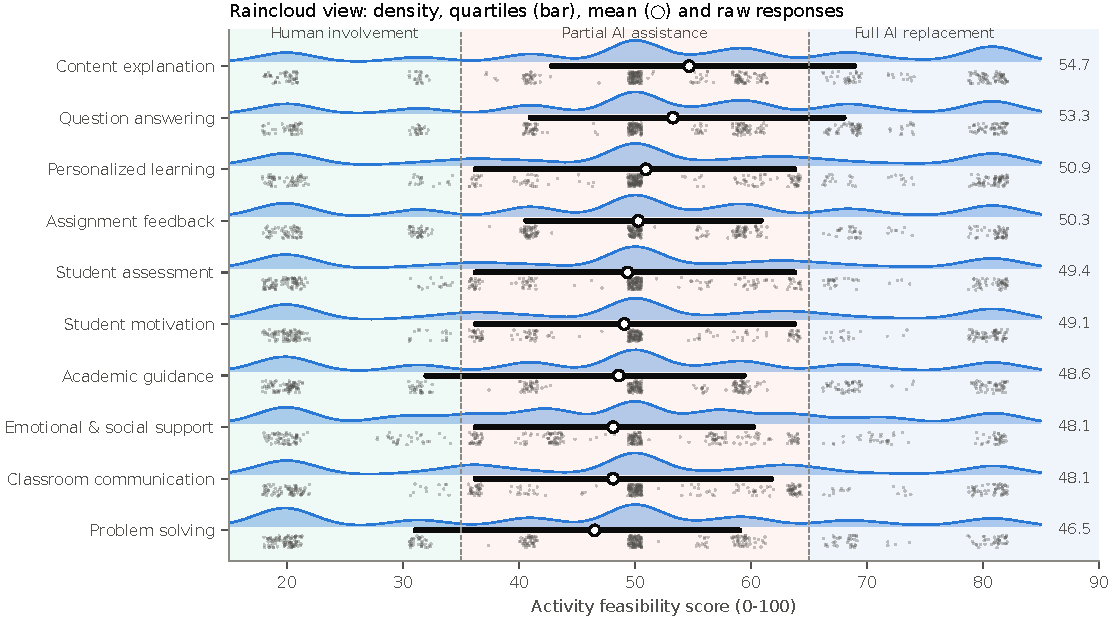
\includegraphics[width=\textwidth]{fig11_activity_raincloud.pdf}
\caption{Raincloud plots of the ten activity feasibility scores: kernel density (cloud), interquartile range (bar), mean (circle) and a random subsample of 400 individual scores per activity (rain). Shaded regions mark the three decision categories.}
\label{fig:raincloud}
\end{figure}

\begin{figure}[!htbp]
\centering
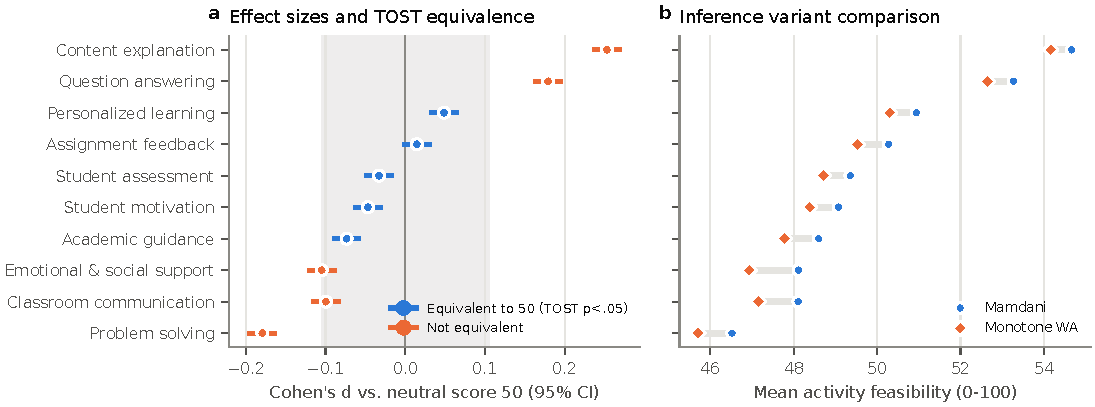
\includegraphics[width=\textwidth]{fig17_effects_and_variants.pdf}
\caption{(a) Cohen's $d_z$ of each activity score against the neutral value 50 with 95\% CIs; the grey band is the TOST equivalence region ($\pm\TostDelta$ points). (b) Mean activity scores under Mamdani and provably monotone weighted-average inference.}
\label{fig:effects}
\end{figure}

\begin{table}[!htbp]
\centering
\caption{Measurement invariance of the eight-factor model: group-wise CFA fit and Tucker's congruence coefficient $\varphi$ (Eq.~\ref{eq:tucker}) between group and pooled loadings (minimum over the eight factors); $\varphi\ge0.95$ indicates factorial equality.}
\label{tab:invariance}
\resizebox{\textwidth}{!}{%
\begin{tabular}{llrccccc}
\toprule
Grouping & Group & $n$ & CFI & RMSEA & SRMR & min $\varphi$ & max $|\Delta\lambda|$\\
\midrule
Gender & Female & 6,476 & 0.939 & 0.053 & 0.048 & 1.000 & 0.03\\
Gender & Male & 5,266 & 0.936 & 0.053 & 0.046 & 1.000 & 0.04\\
Level & Postgraduate & 1,971 & 0.938 & 0.053 & 0.046 & 0.999 & 0.08\\
Level & Undergraduate & 9,856 & 0.939 & 0.052 & 0.046 & 1.000 & 0.01\\
Field & Applied Sciences & 4,274 & 0.939 & 0.052 & 0.045 & 1.000 & 0.03\\
Field & Arts \& Humanities & 1,423 & 0.927 & 0.058 & 0.054 & 0.999 & 0.08\\
Field & Natural \& Life Sciences & 1,291 & 0.939 & 0.055 & 0.047 & 0.999 & 0.05\\
Field & Social Sciences & 4,824 & 0.938 & 0.052 & 0.047 & 1.000 & 0.04\\
Language & Arabic & 448 & 0.930 & 0.062 & 0.049 & 0.987 & 0.15\\
Language & English & 7,422 & 0.939 & 0.052 & 0.046 & 1.000 & 0.03\\
Language & Italian & 501 & 0.924 & 0.060 & 0.056 & 0.993 & 0.16\\
Language & Spanish & 3,046 & 0.937 & 0.056 & 0.051 & 0.999 & 0.07\\
\bottomrule
\end{tabular}}
\end{table}


%======================================================================
\section{Discussion}
\label{sec:discussion}
%======================================================================

\subsection{Answers to the research questions}
\textbf{RQ1 and RQ4: which activities can AI perform?} Students see generative AI as most capable in \emph{content explanation}, \emph{question answering} and, to a lesser extent, \emph{personalised learning}: tasks that consist of retrieving, restructuring and re-expressing codified knowledge. These activities form the AI-leaning end of the partial-assistance band. Activities that require diagnosing an individual's state over time, exercising evaluative judgement or building relationships (assessment, motivation, academic guidance, classroom communication and socio-emotional support) form the human-leaning end. Higher-order problem solving and critical thinking ranks lowest. Although AI can produce solutions, students do not believe it \emph{develops} their own problem-solving, analytical and critical-thinking skills, a concern also voiced in qualitative studies \citep{chantsi2024,chanhu2023}. No activity reached the full-replacement band. This contradicts the expectation of the original proposal that routine activities such as answering repetitive questions would qualify for full replacement. Under current perceptions, even the most automatable teaching tasks call for AI \emph{assistance under human oversight}.

\textbf{RQ2: what drives feasibility?} Reliability is the gatekeeper. It was the strongest unique predictor of the substitution criterion and the largest lever in the fuzzy system, and it was also among the lowest-rated factors. This matches the finding of \citet{ravselj2025} that students value ChatGPT's capabilities but doubt its reliability. Improvements in factual accuracy and verifiability are therefore likely to matter more for substitution feasibility than further gains in fluency or conversational quality. Communication had the smallest unique effect: being easy to talk to does not make an AI a substitute for a teacher.

\textbf{RQ3: can soft computing quantify feasibility?} Yes, with caveats. The hierarchical fuzzy system produced a score that was reliable to compute and convergently and discriminantly valid, robust to its design choices, and fully transparent: each of the 126 rules can be inspected and debated. The ANN matched the best tree ensemble and beat linear regression only by a small margin, and fusing it with the fuzzy outputs did not help. Data-driven models are therefore best used to \emph{validate and calibrate} the interpretable expert system rather than to replace it. The trade-off is clear: the ANN explains about \AnnFisRatio{} times more criterion variance than the untrained fuzzy score, while the fuzzy score explains \emph{why} a given activity is or is not feasible. For policy decisions about delegating teaching work, interpretability is arguably the more important property.

\textbf{RQ5: what are AI's limitations relative to teachers?} The results point to four limitations: (i) unreliable information, the lowest-rated capability factor and the strongest determinant; (ii) weak support for higher-order skill development; (iii) limited capacity for socio-emotional support and classroom interaction, where students fear reduced human contact and social isolation; and (iv) persistent ethical concerns about cheating, plagiarism and privacy. Ethical suitability scored lowest of all factors.

\subsection{Heterogeneity and the mathematical guarantees}
The aggregate result (``partial assistance for every activity'') hides substantial heterogeneity between students. For the AI-enthusiastic third of the sample, AI already approaches or exceeds the full-replacement threshold for explanation, question answering and personalised learning. For the sceptical sixth it remains in the human-involvement band for most activities. Policies that treat students as a homogeneous group will therefore suit neither extreme. Universities may need to offer AI-led options to students who want them while protecting access to human teaching for those who do not. The activity ranking was almost identical across fields of study, and content explanation was rated near the top in every typology. A common core of delegable tasks can therefore guide institutional policy even though the \emph{level} of acceptance varies; the ordering of the remaining tasks depends more on students' general stance towards AI.

The mathematical analysis has a practical corollary. A feasibility score used for decisions should never fall when an AI tool improves on any dimension. The widely used Mamdani scheme does not guarantee this, whereas the weighted-average variant does (Proposition~\ref{prop:monotone}). Because both schemes gave the same conclusions here, we recommend the monotone variant for operational deployment, where scores may be recomputed as tools evolve and must be defensible to stakeholders.

\subsection{The normative--empirical gap on ethics}
Ethical suitability was the second most influential input of the expert rule base but almost irrelevant to students' own substitution judgements. This gap matters for governance. Students' willingness to replace professors by AI is driven by convenience and perceived competence, not by ethical reservations, even though these reservations are widespread. Institutions therefore cannot rely on students' preferences alone to keep AI use within ethical bounds. Explicit policies on disclosure, integrity and data protection remain necessary \citep{unesco2023,cotton2024}. The fuzzy framework makes this normative choice explicit and adjustable: an institution can raise or lower the weight of ethics in FIS$_3$ and see the consequences immediately.

\subsection{Practical implications: a task-level collaboration model}
The results translate into a graded allocation of teaching work:
\begin{itemize}
  \item \textbf{AI-led with human oversight} (explanation, question answering, personalised practice): AI can provide first-line explanations, round-the-clock answers to routine questions and adaptive practice. Teachers curate sources, spot-check accuracy and handle escalations.
  \item \textbf{Shared} (feedback on assignments): AI drafts formative feedback; teachers verify it and add judgement on argument quality and originality.
  \item \textbf{Human-led with AI support} (assessment, motivation, academic guidance, classroom communication, socio-emotional support, higher-order problem solving): teachers remain responsible. AI may support administrative and preparatory sub-tasks, such as generating practice items or summarising student progress, but should not make summative or pastoral decisions.
\end{itemize}
Because reliability is the binding constraint, investments in retrieval-grounded, citation-producing AI tools and in students' verification skills are likely to give the largest returns. The open, vectorised implementation also allows institutions to re-score activities with their own data as AI capabilities and attitudes evolve.

%======================================================================
\section{Limitations and future work}
\label{sec:limitations}
%======================================================================

Several limitations qualify these conclusions. First, the data reflect \emph{students'} perceptions of one AI system (ChatGPT, mostly the free GPT-3.5 version) in late 2023 and early 2024. Perceived capability is not observed teaching performance, teachers' views are not represented, and capabilities are changing rapidly. Second, the survey was not designed for this framework. Some activities, notably student assessment and emotional support, are measured by proxies, and two items form the TSI criterion. Third, the learning-outcome factors (SE, P, AC) are highly correlated and fail the strict Fornell--Larcker criterion, although HTMT supports their distinctness. Fourth, convenience sampling and the over-representation of some countries limit generalisability, although the activity ranking was stable across subgroups. The student typologies are dominated by overall response level (the first principal component explains \TyPC\% of the variance), so they should be read as levels of AI confidence rather than qualitatively distinct profiles. Fifth, the fuzzy rule base, although derived systematically from the proposal and stress-tested, embodies normative choices (e.g.\ the reliability veto and the double weight of pedagogical capability) that other stakeholders may weigh differently.

Future work should (i) collect purpose-built data from both students and teachers, linking perceptions to observed AI performance on authentic teaching tasks; (ii) elicit rule bases from expert panels, for example via Delphi studies, and compare them with data-driven rule learning such as ANFIS \citep{jang1993} or genetic fuzzy systems; (iii) track changes over time with the follow-up waves of the global survey; and (iv) deploy the framework as an interactive decision-support tool for institutions.

%======================================================================
\section{Conclusion}
\label{sec:conclusion}
%======================================================================

This study turned the question ``Can AI replace teachers?'' into a measurable, task-level assessment. A hierarchical fuzzy inference system combined eight validated evaluation factors from more than eleven thousand students in \Ncountries{} countries into an interpretable Teacher Replacement Feasibility Score. Neural and conventional learners were used to validate and benchmark it. Students regard AI as most capable for explanatory and question-answering work and least capable for assessment, motivation, socio-emotional support and the development of higher-order thinking. However, no teaching activity reaches the threshold for full replacement, and reliability is the decisive bottleneck. The future of higher education suggested by these data is therefore not one of teacher replacement. It is one of deliberate human--AI collaboration, in which AI takes on routine explanatory work and human teachers retain responsibility for judgement, motivation, mentoring and care.


\backmatter

\bmhead{Acknowledgements}
The author thanks D.~Rav\v{s}elj, A.~Aristovnik and the Global ChatGPT Student Survey consortium for making their data openly available.

\section*{Declarations}

\begin{itemize}
\item \textbf{Funding:} [This research did not receive any specific grant from funding agencies in the public, commercial, or not-for-profit sectors.]
\item \textbf{Conflict of interest/Competing interests:} The author declares no competing interests.
\item \textbf{Ethics approval and consent to participate:} Not applicable. This study is a secondary analysis of a fully anonymised, publicly available dataset collected with informed consent by the original investigators \citep{ravselj2025}; no new data were collected.
\item \textbf{Consent for publication:} Not applicable.
\item \textbf{Data availability:} The survey data are openly available from Mendeley Data under a CC~BY~4.0 licence \citep{ravselj2024data}.
\item \textbf{Code availability:} The complete analysis code and a runnable Jupyter/Colab notebook are available in the folder \texttt{ai-teacher-feasibility} of \url{https://github.com/isratjahan829/Data-Visualization}.
\item \textbf{Use of generative AI:} [To be completed by the author in line with the journal's policy.]
\item \textbf{Author contribution:} M.B.S.: conceptualization, methodology, software, formal analysis, visualization, writing -- original draft, writing -- review \& editing.
\end{itemize}

\begin{appendices}
\section{Supplementary analysis tables}
\label{app:tables}
This appendix reports every analysis output that is not shown in the main text: item-level descriptive statistics, the compared measurement mappings, the complete fuzzy rule bases, validity correlations, pairwise activity tests, selected ANN hyperparameters, activity-level effect sizes and robustness ranges, subgroup and field-of-study results, quantile-regression coefficients, typology selection and profiles, and country effects. All values are generated directly from the analysis code (\texttt{src/make\_latex.py}).

% generated by src/make_latex.py -- every analysis table not shown in the main text
\begin{figure}[!htbp]
\centering
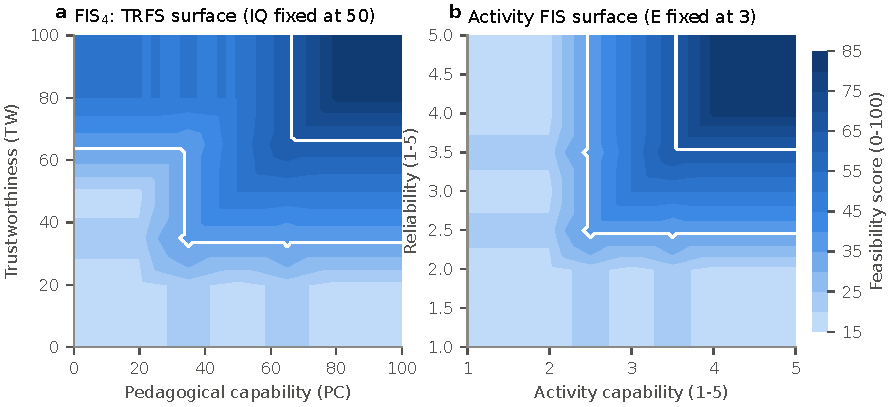
\includegraphics[width=\textwidth]{fig3_control_surfaces.pdf}
\caption{Control surfaces of (a) FIS$_4$ (TRFS as a function of PC and TW, IQ fixed at 50) and (b) the activity FIS (capability $\times$ reliability, ethical suitability fixed at 3). White contours mark the 35 and 65 thresholds.}
\label{fig:A-surfaces}
\end{figure}
\begin{table}[!htbp]
\centering
\caption{Item-level descriptive statistics ($N=\Nfinal$; reverse-coded items marked R). Skew and excess kurtosis are sample estimates; \% agree is the share answering 4 or 5.}
\label{tab:A-items}
\footnotesize
\begin{tabular}{llcccccc}
\toprule
Factor & Item & Mean & SD & Median & Skew & Kurtosis & \% agree\\
\midrule
TE & Q19d & 3.70 & 0.84 & 4 & -0.58 & 0.45 & 64.7\\
TE & Q19f & 3.81 & 0.84 & 4 & -0.64 & 0.65 & 69.3\\
TE & Q19g & 3.81 & 0.84 & 4 & -0.64 & 0.64 & 69.6\\
SE & Q25b & 3.85 & 0.85 & 4 & -0.72 & 0.70 & 71.8\\
SE & Q25c & 3.36 & 1.04 & 3 & -0.35 & -0.39 & 47.9\\
SE & Q25d & 3.59 & 1.01 & 4 & -0.61 & 0.03 & 59.3\\
P & Q26d & 3.33 & 1.03 & 3 & -0.34 & -0.43 & 47.5\\
P & Q26a & 3.67 & 0.89 & 4 & -0.76 & 0.68 & 65.1\\
P & Q26c & 3.67 & 0.91 & 4 & -0.67 & 0.35 & 64.4\\
AC & Q27a & 3.37 & 1.01 & 3 & -0.41 & -0.29 & 49.3\\
AC & Q27b & 3.35 & 1.02 & 3 & -0.38 & -0.32 & 47.8\\
AC & Q26j & 3.56 & 0.99 & 4 & -0.60 & 0.07 & 58.5\\
C & Q19a & 3.62 & 0.85 & 4 & -0.65 & 0.72 & 61.0\\
C & Q19b & 3.63 & 0.90 & 4 & -0.65 & 0.40 & 62.4\\
C & Q19c & 3.40 & 0.97 & 3 & -0.40 & -0.10 & 48.9\\
A & Q19h & 3.25 & 1.01 & 3 & -0.27 & -0.32 & 41.7\\
A & Q19i & 3.59 & 0.94 & 4 & -0.60 & 0.31 & 58.7\\
A & Q19j & 3.51 & 0.94 & 4 & -0.49 & 0.23 & 53.2\\
R & Q19e & 3.28 & 0.92 & 3 & -0.24 & -0.10 & 41.2\\
R & Q24f & 3.34 & 0.94 & 3 & -0.41 & -0.11 & 47.0\\
R & Q24g & 3.16 & 0.97 & 3 & -0.28 & -0.28 & 38.1\\
E & Q22a (R) & 3.08 & 1.13 & 3 & 0.01 & -0.84 & 37.4\\
E & Q22b (R) & 2.84 & 1.24 & 3 & 0.23 & -1.00 & 32.3\\
E & Q22c (R) & 2.85 & 1.23 & 3 & 0.22 & -0.97 & 31.9\\
E & Q22d (R) & 2.99 & 1.16 & 3 & 0.09 & -0.87 & 34.5\\
E & Q22f (R) & 3.29 & 1.11 & 3 & -0.20 & -0.65 & 43.5\\
TSI & Q24b & 2.91 & 1.18 & 3 & 0.02 & -0.95 & 34.6\\
TSI & Q24d & 2.82 & 1.07 & 3 & 0.12 & -0.55 & 25.3\\
\bottomrule
\end{tabular}
\end{table}

\begin{table}[!htbp]
\centering
\caption{Candidate item-to-factor mappings compared before the analysis (TE, SE, P, AC and C items differ; A, R and E fixed). M3 was retained.}
\label{tab:A-mappings}
\footnotesize
\resizebox{\textwidth}{!}{%
\begin{tabular}{lcccccccc}
\toprule
Mapping & $n$ & CFI & TLI & RMSEA & SRMR & min $\alpha$ & min AVE & max HTMT\\
\midrule
M0 (initial a-priori mapping) & 12,066 & 0.883 & 0.865 & 0.070 & 0.060 & 0.595 & 0.324 & 1.004\\
M1 & 12,558 & 0.928 & 0.915 & 0.056 & 0.048 & 0.718 & 0.440 & 0.959\\
M2 & 12,568 & 0.941 & 0.929 & 0.052 & 0.045 & 0.717 & 0.486 & 0.863\\
M3 (final) & 12,564 & 0.940 & 0.928 & 0.052 & 0.045 & 0.718 & 0.487 & 0.806\\
\bottomrule
\end{tabular}}
\end{table}

\begin{table}[!htbp]
\centering
\caption{Complete rule base of FIS$_1$ (pedagogical capability, 81 rules; L/M/H = Low/Medium/High).}
\label{tab:A-rulesPC}
\scriptsize
\resizebox{\textwidth}{!}{%
\begin{tabular}{rccccc|rccccc|rccccc}
\toprule
\# & TE & P & AC & A & PC & \# & TE & P & AC & A & PC & \# & TE & P & AC & A & PC\\
\midrule
1 & L & L & L & L & L & 28 & M & L & L & L & L & 55 & H & L & L & L & L\\
2 & L & L & L & M & L & 29 & M & L & L & M & L & 56 & H & L & L & M & M\\
3 & L & L & L & H & L & 30 & M & L & L & H & M & 57 & H & L & L & H & M\\
4 & L & L & M & L & L & 31 & M & L & M & L & L & 58 & H & L & M & L & M\\
5 & L & L & M & M & L & 32 & M & L & M & M & M & 59 & H & L & M & M & M\\
6 & L & L & M & H & M & 33 & M & L & M & H & M & 60 & H & L & M & H & M\\
7 & L & L & H & L & L & 34 & M & L & H & L & M & 61 & H & L & H & L & M\\
8 & L & L & H & M & M & 35 & M & L & H & M & M & 62 & H & L & H & M & M\\
9 & L & L & H & H & M & 36 & M & L & H & H & M & 63 & H & L & H & H & M\\
10 & L & M & L & L & L & 37 & M & M & L & L & L & 64 & H & M & L & L & M\\
11 & L & M & L & M & L & 38 & M & M & L & M & M & 65 & H & M & L & M & M\\
12 & L & M & L & H & M & 39 & M & M & L & H & M & 66 & H & M & L & H & M\\
13 & L & M & M & L & L & 40 & M & M & M & L & M & 67 & H & M & M & L & M\\
14 & L & M & M & M & M & 41 & M & M & M & M & M & 68 & H & M & M & M & M\\
15 & L & M & M & H & M & 42 & M & M & M & H & M & 69 & H & M & M & H & M\\
16 & L & M & H & L & M & 43 & M & M & H & L & M & 70 & H & M & H & L & M\\
17 & L & M & H & M & M & 44 & M & M & H & M & M & 71 & H & M & H & M & M\\
18 & L & M & H & H & M & 45 & M & M & H & H & M & 72 & H & M & H & H & H\\
19 & L & H & L & L & L & 46 & M & H & L & L & M & 73 & H & H & L & L & M\\
20 & L & H & L & M & M & 47 & M & H & L & M & M & 74 & H & H & L & M & M\\
21 & L & H & L & H & M & 48 & M & H & L & H & M & 75 & H & H & L & H & M\\
22 & L & H & M & L & M & 49 & M & H & M & L & M & 76 & H & H & M & L & M\\
23 & L & H & M & M & M & 50 & M & H & M & M & M & 77 & H & H & M & M & M\\
24 & L & H & M & H & M & 51 & M & H & M & H & M & 78 & H & H & M & H & H\\
25 & L & H & H & L & M & 52 & M & H & H & L & M & 79 & H & H & H & L & M\\
26 & L & H & H & M & M & 53 & M & H & H & M & M & 80 & H & H & H & M & H\\
27 & L & H & H & H & M & 54 & M & H & H & H & H & 81 & H & H & H & H & H\\
\bottomrule
\end{tabular}}
\end{table}

\begin{table}[!htbp]
\centering
\caption{Rule base of the activity-level FIS (27 rules). FIS$_2$ (interaction quality, SE,C$\to$IQ): (L,L)$\to$L; (L,M)$\to$L; (L,H)$\to$M; (M,L)$\to$L; (M,M)$\to$M; (M,H)$\to$M; (H,L)$\to$M; (H,M)$\to$M; (H,H)$\to$H.}
\label{tab:A-rulesAct}
\footnotesize
\begin{tabular}{rcccc|rcccc|rcccc}
\toprule
\# & Cap & R & E & Out & \# & Cap & R & E & Out & \# & Cap & R & E & Out\\
\midrule
1 & L & L & L & L & 10 & M & L & L & L & 19 & H & L & L & L\\
2 & L & L & M & L & 11 & M & L & M & L & 20 & H & L & M & L\\
3 & L & L & H & L & 12 & M & L & H & L & 21 & H & L & H & L\\
4 & L & M & L & L & 13 & M & M & L & M & 22 & H & M & L & M\\
5 & L & M & M & L & 14 & M & M & M & M & 23 & H & M & M & M\\
6 & L & M & H & L & 15 & M & M & H & M & 24 & H & M & H & H\\
7 & L & H & L & L & 16 & M & H & L & M & 25 & H & H & L & M\\
8 & L & H & M & L & 17 & M & H & M & M & 26 & H & H & M & H\\
9 & L & H & H & L & 18 & M & H & H & M & 27 & H & H & H & H\\
\bottomrule
\end{tabular}
\end{table}

\begin{table}[!htbp]
\centering
\caption{Convergent, criterion and discriminant validity of the overall TRFS (Spearman correlations) and known-groups comparison by intensity of use.}
\label{tab:A-validity}
\footnotesize
\begin{tabular}{lccc}
\toprule
Criterion & $n$ & $\rho$ & $p$\\
\midrule
TSI (ChatGPT easier/clearer than professors) & 11,920 & 0.388 & $<$0.001\\
Q24e satisfied with assistance & 11,910 & 0.552 & $<$0.001\\
Q16 overall experience & 11,903 & 0.449 & $<$0.001\\
Q15 intensity of use & 11,898 & 0.301 & $<$0.001\\
Q22h ChatGPT might replace formal education & 11,912 & -0.013 & 0.155\\
\midrule
\multicolumn{4}{l}{\textit{TRFS by intensity of ChatGPT use (Q15): $n$, mean (SD)}}\\
\quad Rarely & 2,481 & 41.6 & (18.2)\\
\quad Occasionally & 3,785 & 48.6 & (18.8)\\
\quad Moderately & 3,484 & 52.8 & (18.7)\\
\quad Considerably & 1,668 & 59.3 & (19.4)\\
\quad Extensively & 480 & 63.5 & (20.5)\\
\bottomrule
\end{tabular}
\end{table}

\begin{table}[!htbp]
\centering
\caption{Wilcoxon signed-rank tests between adjacent activities in the ranking (matched-pairs rank-biserial $r$; Holm-adjusted $p$).}
\label{tab:A-pairwise}
\footnotesize
\begin{tabular}{lcccc}
\toprule
Pair & Mean diff. & $r_{rb}$ & $p$ & $p_{\mathrm{Holm}}$\\
\midrule
A1 vs A2 & 1.40 & 0.317 & $<$0.001 & $<$0.001\\
A2 vs A5 & 2.33 & 0.243 & $<$0.001 & $<$0.001\\
A5 vs A3 & 0.66 & 0.104 & $<$0.001 & $<$0.001\\
A3 vs A4 & 0.92 & 0.084 & $<$0.001 & $<$0.001\\
A4 vs A6 & 0.28 & 0.050 & 0.001 & 0.002\\
A6 vs A8 & 0.48 & 0.088 & $<$0.001 & $<$0.001\\
A8 vs A10 & 0.48 & 0.073 & $<$0.001 & $<$0.001\\
A10 vs A7 & 0.01 & -0.036 & 0.003 & 0.003\\
A7 vs A9 & 1.59 & 0.151 & $<$0.001 & $<$0.001\\
\bottomrule
\end{tabular}
\end{table}

\begin{table}[!htbp]
\centering
\caption{Hyperparameters selected by the inner 3-fold grid search in the \CVfits{} outer folds.}
\label{tab:A-hyper}
\footnotesize
\begin{tabular}{lccc}
\toprule
Model & Hidden layers & $\alpha$ (L2) & Times selected\\
\midrule
ANN (MLP) & (64, 32) & 0.01 & 14\\
ANN (MLP) & (64, 32) & 0.0001 & 7\\
ANN (MLP) & (32, 16) & 0.0001 & 5\\
ANN (MLP) & (32, 16) & 0.01 & 4\\
Hybrid fuzzy-ANN & (32, 16) & 0.0001 & 9\\
Hybrid fuzzy-ANN & (64, 32) & 0.01 & 5\\
Hybrid fuzzy-ANN & (16,) & 0.0001 & 4\\
Hybrid fuzzy-ANN & (16,) & 0.01 & 4\\
Hybrid fuzzy-ANN & (32, 16) & 0.01 & 4\\
Hybrid fuzzy-ANN & (64, 32) & 0.0001 & 4\\
\bottomrule
\end{tabular}
\end{table}

\begin{table}[!htbp]
\centering
\caption{Activity-level effect sizes and robustness: Cohen's $d_z$ against 50 with 95\% CI, TOST $p$ for equivalence within $\pm\TostDelta$ points, 2.5--97.5\% range over \RobDraws{} perturbed fuzzy designs, and the provably monotone weighted-average (WA) score with its \% full / \% human shares.}
\label{tab:A-activity}
\footnotesize
\resizebox{\textwidth}{!}{%
\begin{tabular}{lccccccc}
\toprule
Activity & Mean & $d_z$ [95\% CI] & $p_{\mathrm{TOST}}$ & Equiv. & Perturbation range & WA mean & WA \% full / human\\
\midrule
Content explanation & 54.7 & 0.253 [0.235, 0.271] & 1.000 & no & [48.0, 65.3] & 54.2 & 30.5 / 17.9\\
Question answering & 53.3 & 0.179 [0.161, 0.197] & 1.000 & no & [46.7, 63.8] & 52.6 & 27.3 / 19.5\\
Personalized learning & 50.9 & 0.049 [0.031, 0.067] & $<$0.001 & yes & [44.6, 60.7] & 50.3 & 25.7 / 27.2\\
Assignment feedback & 50.3 & 0.015 [-0.003, 0.033] & $<$0.001 & yes & [44.0, 60.3] & 49.5 & 23.0 / 25.5\\
Student assessment & 49.4 & -0.033 [-0.051, -0.015] & $<$0.001 & yes & [43.3, 59.0] & 48.7 & 23.8 / 29.9\\
Student motivation & 49.1 & -0.047 [-0.065, -0.029] & $<$0.001 & yes & [43.0, 58.4] & 48.4 & 24.0 / 31.9\\
Academic guidance & 48.6 & -0.073 [-0.091, -0.055] & $<$0.001 & yes & [42.6, 58.2] & 47.8 & 20.8 / 28.4\\
Emotional \& social support & 48.1 & -0.105 [-0.123, -0.087] & 0.241 & no & [41.7, 56.8] & 46.9 & 19.8 / 32.1\\
Classroom communication & 48.1 & -0.100 [-0.118, -0.082] & 0.269 & no & [42.0, 57.5] & 47.2 & 21.2 / 34.4\\
Problem solving & 46.5 & -0.179 [-0.197, -0.161] & 1.000 & no & [40.8, 56.1] & 45.7 & 18.1 / 32.5\\
\bottomrule
\end{tabular}}
\end{table}

\begin{table}[!htbp]
\centering
\caption{Overall TRFS by subgroup with Kruskal--Wallis tests and $\varepsilon^2$ effect sizes.}
\label{tab:A-subgroups}
\footnotesize
\begin{tabular}{lccc}
\toprule
Group & $n$ & Mean TRFS & SD\\
\midrule
\multicolumn{4}{l}{\textit{Gender}: $H=52.9$, $p<0.001$, $\varepsilon^2=0.0042$}\\
\quad Female & 6,476 & 49.4 & 19.6\\
\quad Male & 5,266 & 51.9 & 19.8\\
\quad Other & 50 & 45.8 & 20.2\\
\quad Prefer not to say & 106 & 45.9 & 21.1\\
\multicolumn{4}{l}{\textit{Level of study}: $H=35.9$, $p<0.001$, $\varepsilon^2=0.0029$}\\
\quad Doctoral & 516 & 46.1 & 20.3\\
\quad Postgraduate (Master) & 1,455 & 48.8 & 20.0\\
\quad Undergraduate & 9,856 & 50.9 & 19.7\\
\multicolumn{4}{l}{\textit{Field of study}: $H=32.8$, $p<0.001$, $\varepsilon^2=0.0025$}\\
\quad Applied Sciences & 4,274 & 51.8 & 20.1\\
\quad Arts \& Humanities & 1,423 & 49.6 & 19.7\\
\quad Natural \& Life Sciences & 1,291 & 50.1 & 20.3\\
\quad Social Sciences & 4,824 & 49.5 & 19.2\\
\multicolumn{4}{l}{\textit{Mode of study}: $H=13.8$, $p<0.001$, $\varepsilon^2=0.0010$}\\
\quad Blended & 5,389 & 51.2 & 19.9\\
\quad Online & 1,015 & 49.9 & 20.4\\
\quad Traditional & 5,450 & 49.8 & 19.5\\
\multicolumn{4}{l}{\textit{ChatGPT version}: $H=110.8$, $p<0.001$, $\varepsilon^2=0.0092$}\\
\quad Both & 958 & 56.0 & 20.7\\
\quad ChatGPT-3.5 (free) & 10,550 & 49.8 & 19.6\\
\quad ChatGPT-4 (paid) & 384 & 55.5 & 20.0\\
\bottomrule
\end{tabular}
\end{table}

\begin{table}[!htbp]
\centering
\caption{Mean activity feasibility scores by field of study.}
\label{tab:A-field}
\footnotesize
\resizebox{\textwidth}{!}{%
\begin{tabular}{lcccc}
\toprule
Activity & Applied Sciences & Arts \& Humanities & Natural \& Life Sciences & Social Sciences\\
\midrule
Content explanation & 55.3 & 53.4 & 54.5 & 54.4\\
Question answering & 54.2 & 51.5 & 52.8 & 53.1\\
Personalized learning & 52.2 & 50.1 & 50.4 & 50.1\\
Assignment feedback & 51.1 & 49.4 & 50.5 & 49.7\\
Student assessment & 50.4 & 48.5 & 48.9 & 48.7\\
Student motivation & 50.1 & 49.0 & 48.8 & 48.1\\
Academic guidance & 49.9 & 47.9 & 48.0 & 47.7\\
Emotional \& social support & 49.5 & 47.7 & 48.6 & 46.9\\
Classroom communication & 48.8 & 48.3 & 48.2 & 47.3\\
Problem solving & 47.5 & 46.4 & 46.5 & 45.6\\
\bottomrule
\end{tabular}}
\end{table}

\begin{table}[!htbp]
\centering
\caption{Quantile-regression coefficients of the TSI on the TRFS (per 10 points), averaged over \QReps{} jittered replications; OLS: \QolsBeta.}
\label{tab:A-quantile}
\footnotesize
\begin{tabular}{ccc|ccc}
\toprule
$\tau$ & $\beta(\tau)$ & 95\% CI & $\tau$ & $\beta(\tau)$ & 95\% CI\\
\midrule
0.10 & 4.90 & [4.58, 5.23] & 0.55 & 5.70 & [5.43, 5.96]\\
0.15 & 5.34 & [5.02, 5.66] & 0.60 & 5.61 & [5.35, 5.87]\\
0.20 & 5.64 & [5.32, 5.97] & 0.65 & 5.41 & [5.14, 5.67]\\
0.25 & 5.58 & [5.26, 5.90] & 0.70 & 5.23 & [4.94, 5.52]\\
0.30 & 5.48 & [5.17, 5.79] & 0.75 & 5.05 & [4.75, 5.36]\\
0.35 & 5.52 & [5.21, 5.82] & 0.80 & 4.84 & [4.52, 5.16]\\
0.40 & 5.65 & [5.35, 5.95] & 0.85 & 4.92 & [4.56, 5.28]\\
0.45 & 5.68 & [5.40, 5.96] & 0.90 & 4.94 & [4.50, 5.38]\\
0.50 & 5.73 & [5.46, 6.00] & & &\\
\bottomrule
\end{tabular}
\end{table}

\begin{table}[!htbp]
\centering
\caption{Selection of the number of student typologies ($k$-means): mean silhouette, Calinski--Harabasz index and bootstrap stability (mean adjusted Rand index over 20 resamples).}
\label{tab:A-kselect}
\footnotesize
\begin{tabular}{lccc}
\toprule
Solution & Silhouette & Calinski--Harabasz & Bootstrap ARI\\
\midrule
$k=2$ & 0.262 & 5,795 & 0.986\\
$k=3$ & 0.197 & 4,417 & 0.957\\
$k=4$ & 0.149 & 3,535 & 0.935\\
$k=5$ & 0.142 & 2,988 & 0.921\\
$k=6$ & 0.128 & 2,618 & 0.924\\
\bottomrule
\end{tabular}
\end{table}

\begin{table}[!htbp]
\centering
\caption{Profiles of the three student typologies: mean activity capabilities and factor scores (1--5), TRFS and TSI (0--100).}
\label{tab:A-typology}
\footnotesize
\begin{tabular}{lccc}
\toprule
Variable & AI-sceptical & Ambivalent & AI-enthusiastic\\
\midrule
Content explanation & 3.21 & 3.69 & 4.28\\
Question answering & 3.25 & 3.54 & 4.02\\
Assignment feedback & 2.38 & 3.33 & 4.10\\
Student assessment & 2.23 & 3.24 & 4.13\\
Personalized learning & 2.37 & 3.35 & 4.20\\
Student motivation & 2.06 & 3.21 & 4.16\\
Classroom communication & 2.21 & 3.12 & 3.93\\
Academic guidance & 2.07 & 3.16 & 4.05\\
Problem solving & 2.09 & 3.05 & 3.83\\
Emotional \& social support & 2.66 & 3.09 & 3.57\\
TRFS & 30.9 & 46.5 & 66.6\\
TSI & 28.2 & 44.8 & 58.8\\
Teaching effectiveness (TE) & 3.28 & 3.67 & 4.20\\
Student engagement (SE) & 2.82 & 3.50 & 4.15\\
Personalization (P) & 2.67 & 3.44 & 4.19\\
Assessment capability (AC) & 2.30 & 3.31 & 4.18\\
Communication (C) & 3.12 & 3.44 & 3.94\\
Adaptability (A) & 2.65 & 3.36 & 4.01\\
Reliability (R) & 2.59 & 3.17 & 3.75\\
Ethical suitability (E) & 2.68 & 2.95 & 3.28\\
$n$ (\%) & 2,079 (17.4) & 5,885 (49.4) & 3,956 (33.2)\\
\bottomrule
\end{tabular}
\end{table}

\begin{table}[!htbp]
\centering
\caption{Country random intercepts for the TRFS (\MlCountries{} countries with $n\ge\MlMinN$): BLUP of the country mean and deviation $u_c$ from the grand mean.}
\label{tab:A-country}
\scriptsize
\begin{tabular}{lrcc|lrcc}
\toprule
Country & $n$ & Mean & $u_c$ & Country & $n$ & Mean & $u_c$\\
\midrule
Estonia & 123 & 70.9 & +20.2 & Italy & 594 & 49.8 & -0.9\\
Egypt & 493 & 62.4 & +11.8 & Albania & 137 & 49.7 & -1.0\\
Zimbabwe & 64 & 61.7 & +11.0 & Poland & 157 & 49.6 & -1.0\\
Ghana & 227 & 59.7 & +9.1 & Spain & 795 & 49.6 & -1.1\\
Nigeria & 52 & 58.8 & +8.1 & China & 121 & 49.4 & -1.2\\
Bangladesh & 175 & 58.4 & +7.7 & Luxembourg & 117 & 49.1 & -1.6\\
Tanzania & 393 & 57.5 & +6.8 & United Arab Emirates & 58 & 48.9 & -1.7\\
Zambia & 127 & 56.2 & +5.6 & Bosnia \& Herzegovina & 106 & 48.9 & -1.8\\
Algeria & 76 & 56.0 & +5.3 & Latvia & 313 & 48.8 & -1.9\\
Malaysia & 72 & 55.2 & +4.5 & Ecuador & 1362 & 48.7 & -2.0\\
Portugal & 99 & 55.0 & +4.3 & Israel & 167 & 48.2 & -2.4\\
Cape Verde & 37 & 53.6 & +2.9 & Mexico & 675 & 47.3 & -3.4\\
Romania & 585 & 52.6 & +1.9 & Slovakia & 76 & 47.0 & -3.7\\
Chile & 507 & 52.5 & +1.8 & India & 51 & 46.5 & -4.2\\
The Philippines & 293 & 51.8 & +1.1 & Ukraine & 239 & 46.4 & -4.3\\
Croatia & 130 & 51.4 & +0.8 & Russia & 66 & 46.4 & -4.3\\
Hungary & 169 & 51.1 & +0.4 & United Kingdom & 141 & 45.9 & -4.8\\
Bulgaria & 227 & 50.8 & +0.1 & Tunisia & 184 & 45.8 & -4.9\\
Macedonia & 99 & 50.7 & +0.0 & Brazil & 226 & 45.4 & -5.3\\
Greece & 42 & 50.5 & -0.2 & Turkey & 304 & 44.2 & -6.5\\
Cyprus & 255 & 50.3 & -0.4 & Colombia & 116 & 44.1 & -6.6\\
Saudi Arabia & 115 & 50.3 & -0.4 & Guatemala & 65 & 43.6 & -7.1\\
Indonesia & 172 & 50.0 & -0.6 & Palestinian State* & 212 & 43.1 & -7.6\\
Serbia & 130 & 50.0 & -0.7 & Japan & 229 & 40.6 & -10.1\\
Slovenia & 245 & 49.8 & -0.8 & Austria & 168 & 40.0 & -10.7\\
\bottomrule
\end{tabular}
\end{table}

\end{appendices}

\bibliography{refs}

\end{document}
